% -----------------
% abnTeX2: Modelo de Trabalho Academico (tese de doutorado, dissertacao de
% mestrado e trabalhos monograficos em geral) em conformidade com 
% ABNT NBR 14724:2011: Informacao e documentacao - Trabalhos academicos -
% Apresentacao
% -----------------

\documentclass[
	% -- opções da classe memoir --
	12pt,                     % tamanho da fonte
	openright,                % capítulos começam em pág ímpar (insere página vazia caso preciso)
	oneside,                  % twoside para impressão em verso e anverso. Oposto a oneside
	a4paper,                  % tamanho do papel. 
  % -- opções da classe abntex2 --
	% chapter=TITLE,          % títulos de capítulos convertidos em letras maiúsculas
	% section=TITLE,          % títulos de seções convertidos em letras maiúsculas
	% subsection=TITLE,       % títulos de subseções convertidos em letras maiúsculas
	% subsubsection=TITLE,    % títulos de subsubseções convertidos em letras maiúsculas
  % -- opções do pacote babel --
	english,                  % idioma adicional para hifenização
	brazil                    % o último idioma é o principal do documento
]{abntex2}

% --- 
% Pacotes básicos 
\usepackage{lmodern}          % Usa a fonte Latin Modern		>
\usepackage[T1]{fontenc}      % Selecao de codigos de fonte.
\usepackage[utf8]{inputenc}   % Codificacao do documento (conversão automática dos acentos)
\usepackage{lastpage}         % Usado pela Ficha catalográfica
\usepackage{indentfirst}      % Indenta o primeiro parágrafo de cada seção.
\usepackage{color}            % Controle das cores
\usepackage{graphicx}         % Inclusão de gráficos
\usepackage{microtype}        % para melhorias de justificação
\usepackage{colortbl}         % Colorir linhas de tabelas
\usepackage[portuges]{datetime2}
% \DTMlangsetup[portuges]{showdayofmonth=false}
		
% ---
% Pacotes adicionais, usados apenas no âmbito do Modelo Canônico do abnteX2
\usepackage{lipsum}                           % para geração de dummy text

% ---
% Pacotes de citações
\usepackage[brazilian,hyperpageref]{backref}  % Paginas com as citações na bibl
\usepackage[num]{abntex2cite}
\usepackage{float}                            % Citações padrão ABNT

% --- 
% CONFIGURAÇÕES DE PACOTES

% Configurações do pacote backref
% Usado sem a opção hyperpageref de backref
\renewcommand{\backrefpagesname}{Citado na(s) página(s):~}

% Texto padrão antes do número das páginas
\renewcommand{\backref}{}

% Define os textos da citação
\renewcommand*{\backrefalt}[4]{
	\ifcase #1
		Nenhuma citação no texto.
	\or
		Citado na página #2.
	\else
		Citado #1 vezes nas páginas #2.
	\fi}

% Novos comando
\newcommand{\cp}[1]{{\color{orange} [CopyAndPaste] #1}}
\newcommand{\pr}[1]{{\color{blue}[PR] #1}}
\newcommand{\hm}[1]{{\color{red}[HM] #1}}
\newcommand{\todo}[1]{{\color{red}[TO-DO] #1}}

\newcommand{\subItem}[1]{
  {\setlength\itemindent{15pt} \item[-] #1}
}

% ---
% Informações de dados para CAPA e FOLHA DE ROSTO

\titulo{Sistema de Monitoramento de Qualidade de Imunobiológicos na Cadeia de Distribuição e Armazenamento}
\autor{Henrique Martins Miranda}
\local{Campina Grande}
\data{\the\year{}}
\orientador{Paulo Ribeiro Lins Junior}
\newcommand{\instituto}{
  Instituto Federal de Educação, Ciência e Tecnologia\\
  da Paraíba - Campus Campina Grande\\
  Curso Superior de Tecnologia em Telemática
}
\tipotrabalho{Trabalho de conclusão de curso}
% O preambulo deve conter o tipo do trabalho, o objetivo, 
% o nome da instituição e a área de concentração 
\preambulo{Monografia apresentada à Coordenação do Curso de Telemática do IFPB - Campus Campina Grande, como requisito parcial para conclusão do curso de Tecnologia em Telemática.}

\renewcommand{\imprimircapa}{
  \begin{capa}
    \center
    
    \begin{figure}
      \begin{center}
        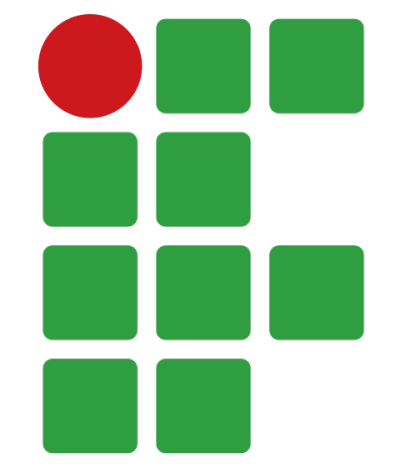
\includegraphics[width=1.8cm]{./assets/logo-ifpb.png}
      \end{center}
    \end{figure}
    
    \ABNTEXchapterfont \large \MakeUppercase{\instituto}
    
    \vspace*{2.5cm}
    
    \ABNTEXchapterfont \large \MakeUppercase{\imprimirautor}
    
    \vfill
    \begin{center}
      \ABNTEXchapterfont \bfseries \large \MakeUppercase{\imprimirtitulo}
    \end{center}
    \vfill
    % \vspace*{6.25cm}

    \large \imprimirlocal
    \par
    \large \imprimirdata
    \vspace*{1cm}
  \end{capa}
}

	
% ---
% Configurações de aparência do PDF final

\definecolor{blue}{RGB}{41,5,195}  % alterando o aspecto da cor azul
\definecolor{orange}{RGB}{255,127,80}

% informações do PDF
\makeatletter
\hypersetup{
  % pagebackref=true,
  pdftitle={\@title}, 
  pdfauthor={\@author},
  pdfsubject={\imprimirpreambulo},
  pdfcreator={LaTeX with abnTeX2},
  pdfkeywords={abnt}{latex}{abntex}{abntex2}{trabalho acadêmico}, 
  colorlinks=true,          % false: boxed links; true: colored links
  linkcolor=black,           % color of internal links
  citecolor=blue,           % color of links to bibliography
  filecolor=magenta,        % color of file links
  urlcolor=black,
  bookmarksdepth=4
}
\makeatother

% --- 
% Espaçamentos entre linhas e parágrafos 

\setlength{\parindent}{1.3cm} % O tamanho do parágrafo

% Controle do espaçamento entre um parágrafo e outro:
\setlength{\parskip}{0.2cm} % Tente também \onelineskip

\makeindex  % Compila o indice

\citebrackets[] % fazer com que as citações dentro do texto virem colchetes

% ---
% Início do documento
\begin{document}
\frenchspacing  % Retira espaço extra obsoleto entre as frases.

% ---
% ELEMENTOS PRÉ-TEXTUAIS
% ---
\pretextual
\imprimircapa
\imprimirfolhaderosto*

% % Isto é um exemplo de Ficha Catalográfica, ou ``Dados internacionais de
% catalogação-na-publicação''. Você pode utilizar este modelo como referência. 
% Porém, provavelmente a biblioteca da sua universidade lhe fornecerá um PDF
% com a ficha catalográfica definitiva após a defesa do trabalho. Quando estiver
% com o documento, salve-o como PDF no diretório do seu projeto e substitua todo
% o conteúdo de implementação deste arquivo pelo comando abaixo:
%
% \begin{fichacatalografica}
%     \includepdf{fig_ficha_catalografica.pdf}
% \end{fichacatalografica}

\begin{fichacatalografica}
  \vspace*{\fill}                 % Posição vertical
  \hrule                          % Linha horizontal
  \begin{center}                  % Minipage Centralizado
    \begin{minipage}[c]{12.5cm}   % Largura

      \imprimirautor

      \hspace{0.5cm} \imprimirtitulo  / \imprimirautor. --
      \imprimirlocal, \imprimirdata-

      \hspace{0.5cm} \pageref{LastPage} p. : il. (algumas color.) ; 30 cm.\\

      \hspace{0.5cm} \imprimirorientadorRotulo~\imprimirorientador\\

      \hspace{0.5cm}
      \parbox[t]{\textwidth}{\imprimirtipotrabalho~--~\imprimirinstituicao,
        \imprimirdata.}\\

      \hspace{0.5cm}
      1. Palavra-chave1.
      2. Palavra-chave2.
      I. Orientador.
      II. Universidade xxx.
      III. Faculdade de xxx.
      IV. Título\\

      \hspace{8.75cm} CDU 02:141:005.7\\

    \end{minipage}
  \end{center}
  \hrule
\end{fichacatalografica}
       % Ficha bibliografica
% \begin{folhadeaprovacao}
  \begin{center}
    {\ABNTEXchapterfont\large\imprimirautor}

    \vspace*{\fill}\vspace*{\fill}
    \begin{center}
      \ABNTEXchapterfont \bfseries \Large \imprimirtitulo
    \end{center}
    \vspace*{\fill}

    \hspace{.45\textwidth}
    \begin{minipage}{.5\textwidth}
      \imprimirpreambulo
    \end{minipage}
    \vspace*{\fill}
    
    % Trabalho aprovado. \imprimirlocal, \today:
  \end{center}

  \assinatura{\textbf{\imprimirorientador} \\ Orientador}
  \assinatura{\textbf{Professor} \\ Membro da Banca}
  \assinatura{\textbf{Professor} \\ Membro da Banca}

  \begin{center}
    \vspace*{0.5cm}
    {\large\imprimirlocal}
    \par
    {\large\imprimirdata}
    \vspace*{1cm}
  \end{center}

\end{folhadeaprovacao}
      % Folha de aprovação
% \begin{dedicatoria}
  \vspace*{\fill}
  \centering
  \noindent
  \textit{Este trabalho é dedicado às crianças adultas que,\\
    quando pequenas, sonharam em se tornar cientistas.} \vspace*{\fill}
\end{dedicatoria}
    % Dedicatória
% \begin{agradecimentos}
Agradeço a minha família, amigos e minha namorada, Jennifer Regina, que me ajudaram e deram apoio na construção deste trabalho. Agradeço também a meu amigo Gledson Santos, que participou ativamente no desenvolvimento dos protótipos citados, aos participantes dos laboratórios de pesquisa Assert e GComPI, que fornecerem local e ferramentas para construção dos protótipos e tiram dúvidas de assuntos que não domino, e por fim, agradeço a todos os professores que tive ao longo do curso.
\end{agradecimentos}
        % Agradecimentos
% \begin{epigrafe}
  \vspace*{\fill}
  \begin{flushright}
    \textit{}
  \end{flushright}
\end{epigrafe}
      % Epígrafe
% resumo em português
\setlength{\absparsep}{18pt} % ajusta o espaçamento dos parágrafos do resumo
\begin{resumo}
  O armazenamento é um dos elementos mais importantes da cadeia de distribuição de vacinas, principalmente pela sensibilidade delas às variações de temperatura, que podem ocasionar diminuição da sua eficácia. Considerando isso, existe uma necessidade de manter constante monitoramento dessa variável, a fim de garantir que o produto final venha a manter suas características originais e a eficiência esperada. Esse trabalho apresenta uma solução baseada em Internet das Coisas, usando comunicação sem fio de baixa potência, para monitorar a qualidade de vacinas, por meio das medidas de temperatura e umidade nos locais de armazenamento. Os dados coletados são organizados em um banco de dados, podendo ser acessados por sistemas decisórios com a finalidade de avaliar a qualidade da vacina antes de sua aplicação, evitando transtornos em decorrência de problemas de armazenamento.

  \textbf{Palavras-chaves}: Monitoramento. Vacinas. IoT. LoRa.
\end{resumo}

% resumo em inglês
\begin{resumo}[Abstract]
  \begin{otherlanguage*}{english}
    Storage is one of the most important components of the vaccine distribution chain, mainly due to its sensitivity to temperature variations, which can cause a decrease in its effectiveness. Considering this, there is a need to keep constant monitoring of this variable, to guarantee that the final product will maintain its original characteristics and the expected efficiency. This work presents a solution based on the Internet of Things, using low power wireless communication, to monitor the quality of vaccines, by measuring temperature and humidity in storage locations. The collected data are organized in a database, which can be accessed by decision systems to assess the quality of the vaccine before its application, avoiding problems due to storage problems.

    \noindent
    \textbf{Key-words}: Monitoring. Vacaciones. IoT. LoRa.
  \end{otherlanguage*}
\end{resumo}
     % Resumos
% ---
% Lista de ilustrações
\pdfbookmark[0]{\listfigurename}{lof}
\listoffigures*
\cleardoublepage

% ---
% Lista de tabelas
\pdfbookmark[0]{\listtablename}{lot}
\listoftables*
\cleardoublepage

% ---
% Lista de abreviaturas e siglas
% \begin{siglas}
%   \item[ABNT] Associação Brasileira de Normas Técnicas
%   \item[abnTeX] ABsurdas Normas para TeX
% \end{siglas}         % Listas

% ---
% Sumario
\pdfbookmark[0]{\contentsname}{toc}
\tableofcontents*
\cleardoublepage

% ---
% ELEMENTOS TEXTUAIS
% ---
\textual

% ---
% Introdução (exemplo de capítulo sem numeração, mas presente no Sumário)
\chapter[Introdução]{Introdução}
\label{cap:intro}
% ---

A saúde é um fator de suma importância para todos os seres vivos, ele é um problema científico, tecnológico, político, prático e filosófico que refere-se a um estado completo de bem estar físico, emocional, social, intelectual e espiritual \cite{almeida2011saude}. 

Segundo o artigo 196 \cite{de2013direito} da Constituição Federal Brasileira a saúde é um direito de todos e dever do Estado garantir medidas políticas sociais e econômicas que visam à diminuição do risco de doenças e de outros agravamentos e ao acesso universal e imparcial às ações e serviços para a sua promoção, proteção e recuperação.

Para garantirmos nossa saúde, precisamos cuidar do nosso corpo e mente, para isto, uma ferramenta que podemos contar são os imunobiológicos, como as vacinas e os soros, diferente de remédios que ajudam no tratamento de pessoas doentes, as imunobiológicos são uma preparação biológica que fornece imunidade total ou parcial de uma determinada doença autoimune para um indivíduo saudável. As vacinas e os soros se diferem pela sua forma de imunização, as vacinas fornece uma imunização ativa, estimulando o nosso organismo na produção de anticorpos, os soros fornecem uma imunização passiva, provendo os anticorpos para o nosso organismo que foram produzidos  em outros organismo \cite{soma2018tratamento}.

Contudo, os imunobiológicos requerem um cuidado elevado para manter a qualidade e sua eficiência, um dos fatores é que são produtos termolábeis, ou seja, se deterioram após determinado tempo expostos a variações de temperaturas e umidade, portanto, é imprescindível assegurar que seu ambiente de armazenagem mantenha uma temperatura e umidade constante \cite{ministerio2001manual} para garantir uma longevidade maior para o produto. Para este propósito, existem a Rede de Frio, um processo desenvolvido pelo Programa Nacional de Imunizações, PNI, de conversação, armazenamento e transporte dos medicamentos, objetivando as condições adequadas dos mesmos, mantendo suas características iniciais \cite{ministerio2001manual}.

No ano de 2014, foi relatado no estudo \cite{oliveira2014avaliaccao} que a qualidade de conservação das vacinas não eram adequadas em boa parte dos municípios da macrorregião Oeste de Minas Gerais, alguns dos motivos citados foram a má gestão dos refrigeradores, falhas no monitoramento da temperatura e insuficiência de recursos humanos. \todo{Falar mais sobre dificuldade no controle de qualidade}

% ---
\section{O Programa Nacional de Imunizações}
\label{intro:PNI}
Com o sucesso da Campanha de Erradicação da Varíola, CEV, iniciada em 1965, tendo seu fim em 1973 \cite{muniz2011memorias}, amplificou dentro do Ministério da Saúde maiores investimento no controle de doenças autoimune, dando um impulso na criação do PNI \cite{temporao2003programa}. O PNI foi fundado com objetivo de controlar e erradicar as doenças imunopreveníveis, através de ações metalizadas de vacinação da população. Em 1980 foi realizada a primeira campanha de vacinação da poliomielite e desde então foram realizadas diversas campanhas, tais como a da rubéola, sarampo, tuberculose febre amarela \cite{temporao2003programa, ministerio2001manual} e atualmente contra a COVID-19.

De acordo com a Lei n.º 6.259 de 30 de outubro de 1975, regularizada pelo Decreto nº 78.231 em 1976, certificar o PNI, sobre a responsabilidade do Ministerio da Saúde e define as seguintes competências \cite{ministerio2001manual}:

  \begin{itemize}
    \item implantar e implementar as ações do Programa, relacionadas com as vacinações de caráter obrigatório;
    \item  estabelecer critérios e prestar apoio técnico e financeiro à elaboração, implantação e implementação dos programas de vacinação a cargo das secretarias de saúde das unidades federadas;
    \item estabelecer normas básicas para a execução das vacinações;
    \item supervisionar, controlar e avaliar a execução das vacinações no território nacional, principalmente o desempenho dos órgãos das Secretarias de Saúde, encarregados dos programas de vacinação.
  \end{itemize}

% ---
\section{Rede de frio}
\label{intro:redes-de-frio}
A Rede de Frio, também chamado de Cadeia de Frio é um processo definido pelo PNI designado a auxiliar os profissionais da área da saúde, responsáveis pela imunização no Brasil para que possa assim, garantir a efetividade e durabilidade dos imunobiológicos e medicamentos termolábeis.

No Manual de Rede de Frio \cite{ministerio2001manual} é definido os requisitos dos ambientes de armazenagem para garantir a efetividade dos produtos, desde os laboratórios produtor as instâncias locais, passando pela instância nacional, estadual, e no transporte entre eles. Para as  Câmaras frigoríficas, a temperatura de operação é entre -20°C a +2°C, variando conforme o material armazenado, para a maioria dos imunobiológicos o recomendado é de +2°C e +8°C para ter um melhor controle da sua validade, havendo algumas exceções, como por exemplo, as vacinas Pfizer-BioNTech e Moderna,  produzidas para combater o COVID-19, que precisam ser armazenadas entre –80°C a –60°C e –25°C e –15°C, respectivamente \cite{niforatoscommon}.

% ---
\section{Justificativa e Relevância do Trabalho}
\label{intro:justificativa}
Atualmente, com o início da distribuição das vacinas contra o COVID-19 em todo o mundo, uma das dificuldades enfrentadas é o controle de qualidade no armazenamento tanto em transporte \cite{baechallenges}, quanto no local da aplicação justamente por serem produtos sensíveis a temperatura e necessitarem de muita cautela, em contrapartida, por ser um produto com uma demanda elevada, a sua oferta deve ser rápida para que haja imunização em massa da população, encaminhando-se para o fim da pandemia.

Esses desafios enfrentados na distribuição das vacinas do COVID-19 não são exclusivamente deles, enfermeiras de Minas Gerais, com o objetivo de inteirar-se acerca do sistema de manutenção dos produtos, realizaram um estudo sobre a conservação de vacinas em unidades básicas de saúde, UBSs. Nessa pesquisa foi relatado diversas irregularidades no armazenamento dos materiais termolábeis sem o comprimentos das normais da PNI, como por exemplo, a presença de vacinas que deveriam ter sido descartadas por terem atingido seu tempo máximo de diluição, ainda presentes nos refrigeradores, cerca de 52\% dos imunobiológicos armazenados nos refrigeradores eram estabelecidos erroneamente e 36\% dos refrigeradores observados contavam com objetos portas como fracos vazios.

Analisando as temperaturas dos ambientes de armazenagem, foi observado que 4\% das unidades não realizavam o registro da temperatura dos refrigeradores, 88\% dos refrigeradores usavam termômetros analógicos de baixa confiabilidade e cerca de 12\% foram analisados na hora da visita temperaturas abaixo da faixa recomendada (+2°C a +8°C), chegando a 0°C, outros estudos realizado \cite{oliveira2014avaliaccao, nelson2007monitoring, falcon2020vaccine} também testemunharam essa irregularidade na temperatura em seus respectivos locais ao longo do mundo, valendo salientar o estudo realizado na Bolívia \cite{nelson2007monitoring}, que teve resultados ainda piores, sendo registado um temperatura mínima de -7.2°C e uma máxima de 22.7°C.

Pensando nesse cenário, esse trabalho apresenta uma alternativa para melhorar a forma de monitoramento de temperatura e umidade realizadas de produtos imunobiológicos por laboratórios, unidades públicas de saúde e afins no intuito de auxiliá-los a manter os materiais em suas em suas melhores condições.

% ---
\section{Objetivos}
\label{intro:objetivos}

\subsection{Objetivo Geral}
\label{intro:objetivos:geral}
Construir uma arquitetura baseada em conceitos de IoT visando o monitoramento de temperatura e umidade de imunobiológicos para auxiliar funcionários da saúde, garantindo melhores condições para a vacinação da população frente a incidência de doenças.

\subsection{Objetivos Específicos}
\label{intro:objetivos:especificos}
\begin{itemize}
  \item Construir um protótipo inicial para coleta da temperatura e umidade nos ambientes de armazenagens dos imunobiológicos.
  \item Implementar um servidor para a armazenagem dos dados coletados e posteriormente fornecer históricos das temperaturas e umidade ao aplicativo móvel.
  \item Desenvolver um aplicativo móvel para fornecer uma interface amigável para os usuários auxiliando no controle de qualidade dos produtos.
  \item Realizar testes e análises dos dados de transmissões a fim de garantir a confiabilidade das temperaturas e umidade coletadas.
\end{itemize}

% ---
% \section{Metodologia}
% \label{intro:metodologia}

% No intuito de alcançar os objetivos pretendidos, a metodologia utilizada neste trabalho foi composta pelas seguintes etapas:

% \begin{itemize}
%   \item \todo{Adicionar os pontos}.
% \end{itemize}

% ---
\section{Estrutura do Documento}
\label{intro:estrutura}

Os capítulos subsequentes estão organizados da seguinte maneira:

\hm{A ser feito quando o documento tiver pronto}
\chapter{Fundamentação Teórica}
\label{cap:fundamentacao}
Neste capítulo serão abordados os principais conceitos e tecnologias utilizadas no desenvolvimento deste projeto, do hardware à aplicação móvel, iniciando pelo conceito principal, a Internet das Coisas.

% ---
\section{Internet das Coisas}
\label{fund:iot}
Com o intuito de ampliar a internet atual, interligando os objetos do nosso cotidiano, animais e humanos em uma única rede, foi criado a Internet das Coisas, IoT, também conhecida como internet de todas as coisas. Para tal, os objetos viram objetos inteligentes, possuindo capacidade de comunicação associados com sensores que fornecem dados para outros dispositivos. Estes aparelhos, conectados a IoT, se comunicam via internet, trocando dados em tempo real, transmitindo informações acerca do ambiente que estão inseridos e/ou até mesmo dos seus respectivos estados. 

Deste modo, é adicionando uma nova gama de possibilidades, trazendo grandes benefícios para ambientes domésticos, mas principalmente para a zona industrial. No primeiro caso, aplicações, tais como: aprendizagem reforçada, monitoramento e vigilância inteligentes e vida assistida, têm despontado entre aquelas que mais chamam atenção, tanto dos usuários, como das empresas de desenvolvimento de soluções tecnológicas. No segundo caso, IoT se apresenta como um diferencial competitivo importante em campos, com a automação e manufatura industrial, logística, gestão de processos de negócio, etc.

Do ponto de vista da produtividade, IoT apresenta-se como um importante meio pelo qual pode-se desenvolver aplicações sofisticadas que podem integrar o mundo real e o mundo virtual. Em empresas de manufatura, produtos conectados permitem a existência de um ambiente de serviços e produtos no qual a manutenção pode ser realizada com base na necessidade real, em vez de uma suposição estatística. Adicionalmente, produtos e máquinas conectados podem receber atualizações de software quando disponíveis, para garantir que estejam sempre funcionando em eficiência ótima.

% ---
\section{Protocolos de Comunicação}
\label{fund:protocolos}
Protocolos de comunicação são conjuntos de normas que definem uma forma de troca de mensagens entre dois ou mais dispositivos em um determinado meio físico. Os meios mais comuns são por cabos de materiais condutores e pelo ar, transmitindo ondas eletromagnéticas, na IoT o que se predomina é por meio sem fio (\textit{wireless}). Neste projeto, foram utilizados dois protocolos de comunicações, o LoRa e o HTTP.

% ----
\subsection{LoRa}
\label{fund:lora}
A tecnologia Long Range, LoRa, é uma forma de comunicação sem fio, semelhante ao Wi-Fi e ao Bluetooth, que permite um longo alcance de comunicação com baixo custo. O raio de comunicação sem fio utilizando o LoRa, dependendo do dispositivo selecionado, pode alcançar quilômetros de distância.

Embora o LoRa tenha sido fundamentalmente desenvolvido pela Semtech Corporation, seu padrão imposto pelo LoRa permitiu que muitas empresas a utilizassem para diversos projetos com um custo benefício satisfatório, aumentando o ecossistema e ganhando um envolvimento significativamente maior, uma variedade superior de produtos e um acréscimo geral no uso e aceitação. 

O LoRa em si diz respeito à camada física, sendo a camada lógica é chamada de LoRaWAN, um protocolo usado pelo LoRa para comunicação entre pontos de conexões de um nós final (\textit{End Nodes}) para envios de informações diretamente a um concentrador (\textit{Gateway}), que centraliza as informações e envia a um determinado sistema \cite{lora2021specification}. Os End Nodes são dispositivos responsáveis por coletar os dados necessários e transmiti-los a um determinado Gateway, o Gateway por sua vez, é responsável por receber as informações de múltiplos End Nodes e repassá-lo a um determinado sistema, por exemplo um servidor onde será armazenado esses dados, como podemos ver na figura \ref{fig:end-nodes-gateways}.

\begin{figure}[H]
  \centering
  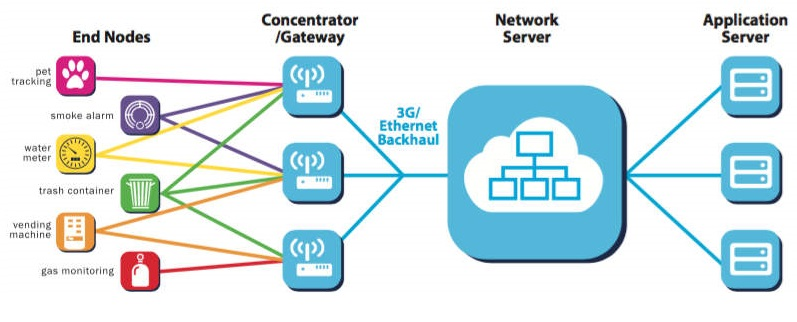
\includegraphics[width=.80\textwidth]{assets/lora-network-architecture.png} 
  \caption{Representação da relação entre os dispositivos LoRa (Adaptada de \cite{lora2021architecture}).}
  \label{fig:end-nodes-gateways} 
\end{figure}

% ----
\subsection{HTTP/HTTPS}
\label{fund:http}
Inicialmente utilizado pelo \textit{World-Wide Web}, WWW, em 1990, como o protocolo base da internet por ser uma protocolo leve e rápido para transições de informações em sistemas distribuídos, o \textit{Hypertext Transfer Protocol}, HTTP, é um protocolo que tramite documentos de diversos formatos através da sistemas distribuídos, mais conhecido pela sua disseminação pela internet \cite{berners1996hypertext}. Quanto anos depois, em 1994, a Netscape Communications criou o HTTPS, uma implementação do HTTP adicionando uma nova camada, a de segurança, utilizando-se do protocolo SSL/TLS, um protocolo que fornece segurança entre comunicações sobre rede de computadores.

O HTTP funcionando baseado no paradigma de cliente e servidor, onde o cliente estabelece uma conexão fazendo uma requisição solicitando algo ao servidor, e o servidor, por sua vez, o responde enviando uma mensagem.  Tais requisições possuem um método atrelado a ele, esses métodos são usados semanticamente, com o objetivo de organizar e dividir suas responsabilidades, os métodos mais utilizados são: GET, POST, PUT e DELETE. o GET é usado quando o cliente solicita dados ao servidor, o POST quando o cliente quer enviar alguma nova informação, o PUIT é semelhante ao POST, entretanto, é referente a atualização de um dados existente e o DELETE é uma requisição pedindo a remoção de uma determinada informação \cite{mozilla2019http}.

Essas mensagens que transitam entre clientes e servidores, são compostas por linhas de textos divididas em três blocos como pode ser visto na figura \ref{fig:post-request}. O primeiro bloco consiste em uma linha com o método da requisição, a url, ou seja, o caminha do documento seguido pela a versão do protocolo; o segundo bloco é referente ao cabeçalho HTTP, responsável por fornecer informações e metadados ao servidor, como o tipo de dado transitado ou dados que alteram seu comportamento; o terceiro bloco é respectivo ao bloco de dados, este bloco é opcional, dependendo do tipo de requisição realizada, mais utilizado pelos métodos POST e PUT.

\begin{figure}[H]
  \centering
  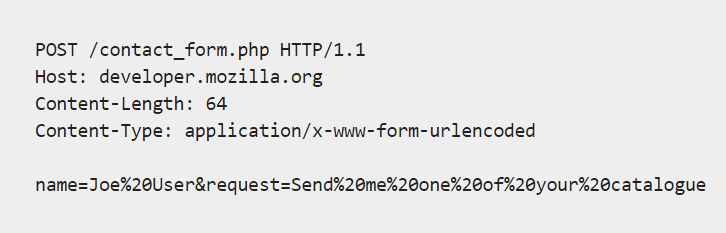
\includegraphics[width=.80\textwidth]{assets/post-request.png} 
  \caption{Exemplo de uma requisição POST (Retirado de \cite{mozilla2019http}).}
  \label{fig:post-request} 
\end{figure}

% ---
\section{Plataformas de Prototipagem}
\label{fund:plataforma-proto}
Plataformas de prototipagem eletrônica são formas facilitadas de desenvolver um protótipo inicial de determinado projeto. Uma das plataformas de prototipagem existentes mais famosa é o Arduino, uma plataforma de código aberto criada em 2005 na Itália pelo professor Massimo Banzi, que tinha como objetivo, ensinar eletrônica e programação para seus alunos, provendo uma forma acessível e de fácil uso. O Arduino possui seu próprio ambiente de desenvolvimento de mesmo nome, utilizando de sua linguagem de programação baseada em C.

Outra plataforma bem conhecida é a família de microcontroladores ESP, e assim como suas concorrentes, oferece módulos de baixo custo e versáteis para várias soluções tecnológicas, dos quais destacam-se a série ESP32. Tal série, acabou sendo mais conhecida pelas suas variações de modelos feitas por empresas distintas, cada modelo possuindo seus diferenciais, como por exemplo o modelo da Heltec Automation, que inclui conectividades com WiFi, bluetooth e LoRa.

% ---
\section{Sensor DHT-22}
\label{fund:dht-22}
O sensor DHT-22 é um sensor de temperatura e umidade da família de sensores DHT comumente utilizado em aplicações de IoT por ser um sensor pequeno(como podemos ver na figura \ref{fig:dht-22}) e possuir um baixo custo. Ele opera na faixa de 3.3 a 6 Volts e consegue capturar dados de temperatura entre -40°C a 80°C e umidade entre 0\% a 100\% RH, com uma acurácia de 0.5°C e 2\% RH, respectivamente \cite{datasheetDHT22}.

\begin{figure}[H]
  \centering
  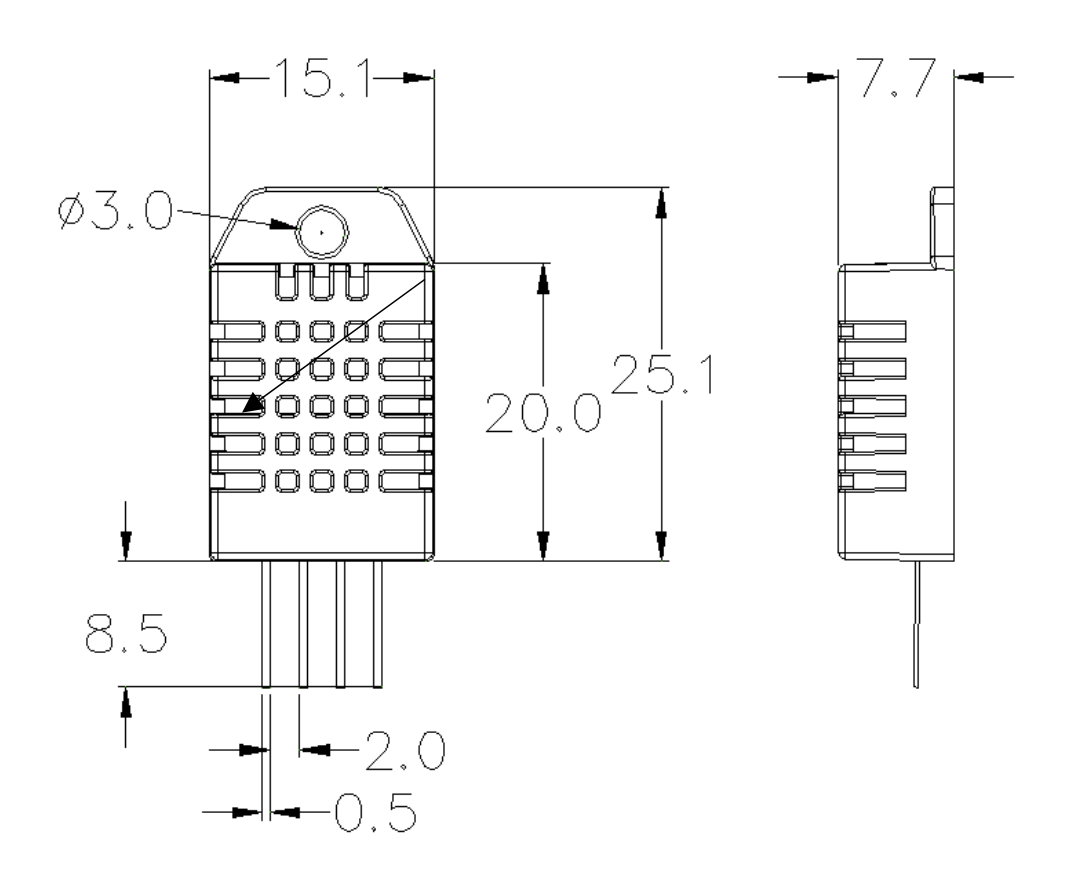
\includegraphics[width=.80\textwidth]{assets/dht-22.png} 
  \caption{Dimensões em milímetros do sensor DHT-22 (Retirado de \cite{datasheetDHT22}).}
  \label{fig:dht-22} 
\end{figure}

% ---
\section{Servidor}
\label{fund:servidor}
Um servidor é um sistema de computação centralizada, responsável por fornecer serviços em uma rede de computadores. Esses serviços variam conforme a necessidade do sistema, podendo ser um controlador de domínio, provedor de arquivos, de impressão, de e-mails entre outros. No modelo cliente/servidor (figura \ref{fig:client-server-model}), por sua vez, o servidor é responsável por receber as requisições de clientes, provendo informações e dados de acordo com a demanda.

\begin{figure}[H]
  \centering
  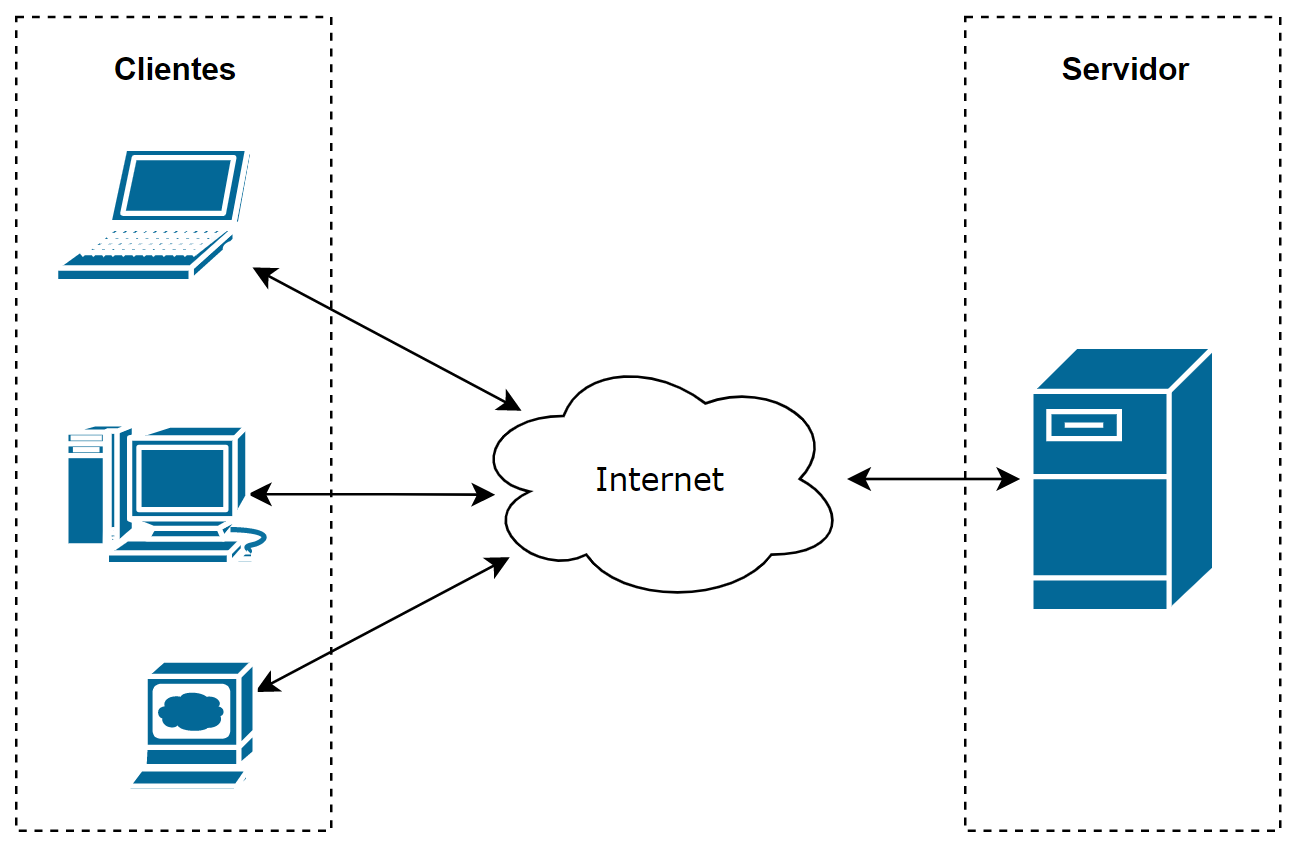
\includegraphics[width=.80\textwidth]{assets/client-server-model.png} 
  \caption{Representação do modelo cliente/servidor (Autoral).}
  \label{fig:client-server-model} 
\end{figure}

% ----
\subsection{Node.js}
\label{fund:node}
Em 2009, Ryan Dahl criou o Node.js ou simplesmente Node, um ambiente de código aberto de execução Javascript para ser utilizado por servidores (\textit{server-side}) baseado no interpretador V8 da Google. O objetivo do Node é fornecer uma forma de criar serviços com alta capacidade de escala, consumindo pouca memória e de fácil aprendizado. Apesar da linguagem de programação Javascript fornecer uma performance inferior às linguagens já existentes para esse objetivo, seu uso oferece dois grande benefícios, ser uma linguagem de fácil aprendizado e de grande uso por ser a linguagem padrão dos navegadores, e consequentemente do desenvolvimento web \cite{tilkov2010node}.

A forma de execução no Node é por eventos assíncronos, diferente da maioria dos outros ambientes modernos que utilizam threads do sistema operacional, SO. O Node usa apenas uma thread assíncrona principal que executa operações de entrada e saída de dados, E/S, chamada de \textit{Event Loop} \cite{nodejsAbout}. O \textit{Event Loop} funciona em um ciclo, escutando uma lista de chamas, onde são armazenadas as requisições recebidas, e as direcionando cada uma para uma Thread a parte, que executará a função recebida, como podemos ver na figura \ref{fig:event-loop-node}. A priori, o  Node possui quatro Threads trabalhadoras, responsáveis por executar as funções, entretanto, é possível configurar, dependendo da máquina, onde está sendo efetuado a instância do Node.

\begin{figure}[H]
  \centering
  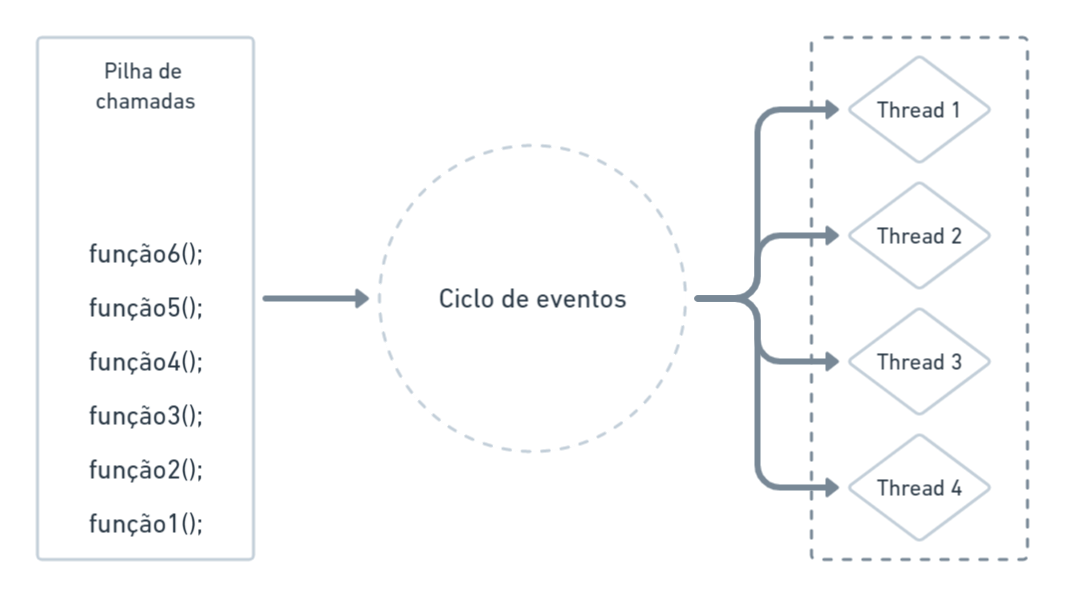
\includegraphics[width=.80\textwidth]{assets/event-loop-node.png} 
  \caption{Ciclo de eventos no Node (Autoral).}
  \label{fig:event-loop-node} 
\end{figure}

% ----
\subsection{InfluxDB}
\label{fund:influxdb}
O InfluxDB é um banco de dados que armazena séries temporais (\textit{data series database}), ou seja, sua chave é o tempo e sua forma de armazenagem de dados é em ordem cronológica. Ele foi projetado para lidar com grandes cargas de escrita e consulta, perfeito para armazenar dados em tempo real, como monitoramento de DevOps, métricas de aplicativos, big data e dados de sensores da IoT \cite{giacobbe2018implementation}. De forma geral, séries temporais acabam se tornando gráficos em função do tempo em um determinado período, por exemplo a temperatura de um freezer ao decorrer do dia, podendo assim ver facilmente a máxima, a mínima e suas variações. Esses dados podem ser também coletados e feito uma análise mais complexa usando qualquer ferramenta estatística, dependendo da sua necessidade.

O InfluxDB é composto por \textit{databases} (bancos de dados), \textit{measurements} (medições), \textit{fields} (campos) e \textit{tags}. Podemos representar essa estrutura como conjuntos como podemos ver na figura \ref{fig:influxdb-struct}, no InfluxDB é possível ter inúmeros \textit{databases}, onde cada \textit{database} contém suas \textit{measurements} que são tabelas de dados correspondentes a algum dado em específico. Por exemplo, se tivermos 2 sensores que coletam dados diferentes, cada sensor viraria um \textit{measurement}, e cada \textit{measurement} é composto  de dois tipo de atributos, os \textit{fields}, onde ficam os dados da sua medida, e as \textit{tags}, que são campos de dados que diferem \textit{fields} por serem campos indexáveis, feitos exclusivamente para realizar buscas, tal como, é comum adicionar uma \textit{tag} que seja um identificador do dispositivo que coletou esse medida.

\begin{figure}[H]
  \centering
  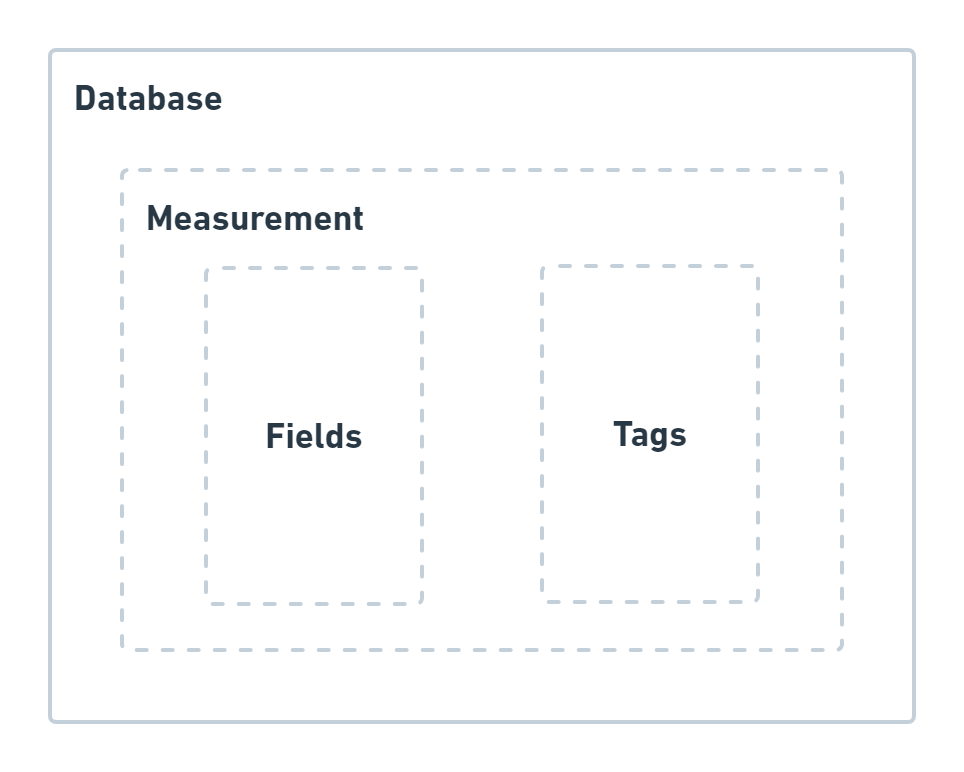
\includegraphics[width=.80\textwidth]{assets/influxdb-struct.png} 
  \caption{Composição de um banco de dados do InfluxDB (Autoral).}
  \label{fig:influxdb-struct} 
\end{figure}

% ----
\subsection{Docker}
\label{fund:docker}
Docker é uma plataforma \textit{open source}, desenvolvida utilizando a linguagem de programação GO pela Google, com o objetivo de criar facilmente  ambientes isolados (containers) com um alto desempenho e portáteis, sendo uma opção em relação às virtualizações. Desta maneira, é possível, por exemplo, criar inúmeras aplicações usando as mesmas tecnologias, cada uma em um \textit{container} diferente e nenhuma vai interferir na outra, e todas na mesma máquina. Se for preciso replicar em outra máquina, é possível criar uma imagem do container e instalar o mesmo ambiente nesta outra máquina.

Em comparação com as virtualizações, os containers não precisam de um sistema operacional, apenas o essencial para executar determinada função. Dessa forma, os containers conseguem ter um controle maior, consomem menos recursos, ganham uma maior flexibilidade e uma manutenibilidade. Podemos ver a comparação entre virtualização e containers na figura abaixo.

Apesar dessa facilidade que containers trazem consigo, gerenciar vários ao mesmo tempo pode ser bem trabalhoso, para isto, foram criados os orquestradores de containers, se baseando em orquestradores de orquestras sinfônicas, que rege o comportamento da sua banda durante uma determinada apresentação. Tais orquestradores auxiliam na organização dos containers, informando que devem iniciar primeiro, quais são as dependências de cada um, interligam suas redes se preciso, entre outras funcionalidades. Para o Docker, um dos orquestradores mais utilizados é o Docker Compose.

\begin{figure}[H]
  \centering
  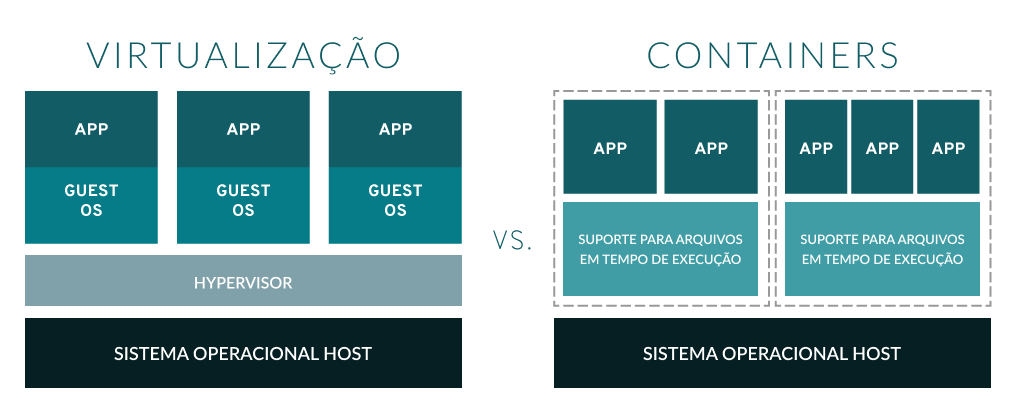
\includegraphics[width=.80\textwidth]{assets/virtualization-vs-containers.png} 
  \caption{Comparação entre o modelo de virtualização e modelo de containers (Adaptada de \cite{redhat2020Containers}).}
  \label{fig:virtualization-vs-containers}
\end{figure}

% Referencias
% - https://www.opservices.com.br/o-que-e-docker/
% - https://www.meupositivo.com.br/panoramapositivo/container-docker/
% - https://www.treinaweb.com.br/blog/no-final-das-contas-o-que-e-o-docker-e-como-ele-funciona/

% ---
\subsection{Computação em Nuvem}
\label{fund:nuvem}
Há uma crescente demanda por serviços de Tecnologia em Informação, TI, ofertados através da Internet, incluindo armazenamento de dados, hospedagem de sites, softwares, banco de dados, rede entre outros. Este fornecimento de serviços de computação, via Internet, é chamado de computação em nuvem. Tal crescimento vem das diversas vantagens oferecidas pela computação em nuvem, como uma disponibilidade maior, recursos flexíveis, normalmente se pagando apenas o usado, trazendo assim, uma redução no custo, possibilidade de escalonamento de acordo com as necessidades da empresa, não precisar gastar nem se preocupar com a infraestrutura entre outras \cite{sousa2009computaccao}.

% ---
\section{Aplicativo Móvel}
\label{fund:app}
Aplicativo móvel, APP, é um \textit{software} desenvolvido especificamente para dispositivos móveis, como telefones celulares, tablets, relógios inteligentes entre outros. Cada SO utiliza uma determinada linguagem de programação para desenvolvedores poderem criar os apps. Com uma grande diversidade de sistemas operacionais, com uma linguagem de programação distintas, transformam o desenvolvimento de aplicativos multiplataformas mais trabalhoso e repetitivo, pois tem que ser programada uma versão diferente para cada plataforma. Tendo esse problema em mente, várias formas de programação híbridas foram criadas, com o princípio de poder programar utilizando apenas um código para várias plataformas distintas, dentre elas, as duas que mais se destacam atualmente são o Flutter e o React Native.

% ----
\subsection{React Native}
\label{fund:react-native}
O React Native é um \textit{framework} para desenvolvimento nativo voltado para dispositivos para os dois principais SO móveis atualmente, Android e iOS. Ele dispõe de um código aberto, mantido pelo Facebook e sua comunidade. É um \textit{framework} bastante popular, utilizado por grandes empresas globais atualmente, como Netflix, Uber, a própria Facebook e empresas brasileiras como o EBANX e a Globo \cite{empresasbrreact}.

O React Native utiliza a linguagem JavaScript como principal e a renderiza para código nativo, para isso é adicionado uma camada em JavaScript, chamada de \textit{Bridge} que se comunica com o sistema operacional, mandando comandos para renderizar os componentes nativos \cite{docreactnative}.

% ---
\section{Trabalhos Relacionados}
\label{fund:trabalhos-relacionados}
Estudantes do Instituto Federal da Bahia desenvolveram uma pesquisa \cite{cruzdesenvolvimento} sobre diferentes métodos de construção de um sensor de temperatura de baixo custo voltado para o monitoramento de vacinas, pois a temperatura é uma das variantes de grande importância no  processo de conservação de materiais imunobiológicos.

No estudo \cite{lima2019controle}, foi desenvolvido um produto de monitoramento de temperaturas de caixas térmicas usadas no transporte de materiais termolábeis, com o  objetivo de alertar os transportadores de quando a condição de armazenagem estiver fora da faixa ideal, disposdo de sinais auditivos e visíveis. No seu protótipo foi utilizado uma tela LCD para visualizar a temperatura atual, um led vermelho e outros verde para informar visivelmente sobre a condição do ambiente, um sensor de temperatura DS18B20, para coletar os dados necessários e um Arduíno Uno R3, como controlador dos equipamentos.

Em \cite{kersbaum2019monitoramento}, um estudo similar ao citado posteriormente, foi construído um dispositivo de baixo custo para o monitoramento de temperaturas voltado para geladeiras domésticas que armazenam vacinas em municípios do Brasil de pequeno porte, pois possuem baixa quantidade de insumo que consequentemente, seus ambientes de armazenagem de materiais termolábeis são precários, possuindo poucas câmeras específicas para armazenagem deste tipo de material, que acabam utilizando geladeiras domésticas. Seu protótipo é composto por um Arduino conectado a uma célula de Peltier, refrigerado por ventoinhas acoplado em uma caixa de isopor, os dados da temperatura são coletados pelo Arduino e enviado para um computador onde pode ser visualizado por um web site e armazenado em uma planilha excel.

Na dissertação de Mestrado de Lopes Neto \cite{lopes2019monitoramento}, foi desenvolvido uma plataforma em Arduino para transmissão de dados de temperatura do interior dos ambientes gerais de conservação de materiais sensíveis à temperatura, transmitido via SMS e GPRS para uma central onde é armazenado os dados para consultas posteriores.

Tendo em vista as pesquisas mencionadas acima, venho através deste trabalho, contribuir para uma solução mais completa, de baixo custo e energeticamente eficaz, utilizando tecnologias modernas e escaláveis, com o intuito de auxiliar os profissionais da saúde no controle dos imunobiológicos.
\chapter{Metodologia}
\label{cap:metodologia}
O sistema proposto neste projeto, se refere a uma plataforma que fornece tanto os dispositivos para a captação dos dados dos imunobiológicos, quanto ao sistema em nuvem para armazenagem dos dados e de um aplicativo móvel para a gerência e análise das informações, seguindo a mesma estrutura representada na figura \ref{fig:end-nodes-gateways} na sessão \ref{fund:lora}, de modo a fornecer aos usuários, um produto  de fácil uso para monitorização de temperatura e umidade, possibilitando o histórico dos dados coletados em um determinado cliente.

Podemos então, separar este sistema em quatro partes, cada uma delas com uma determinada função, elas são, end-node, gateway, servidor e aplicativo móvel. Mas antes, para uma visão geral, vamos ver como foi estruturado o envio de pacotes entre cada etapa.

% ---
\section{Estrutura dos Pacotes}
\label{metod:pacotes}
Definir um padrão de transmissão dos pacotes é de suma importância para facilitar a identificação dos dados e ajuda no reconhecimento de possíveis erros que possam ocorrer na transmissão dos dados.

Dentre a comunicação do gateway, servidor e o aplicativo móvel, que utiliza o protocolo HTTP, existem vários padrões de transmitir dados já definidos e consolidados pela comunidade,  um dos mais utilizados é o \textit{JavaScript Object Notation}, JSON, um formato leve e de código aberto, se baseando na estrutura de objetos do JavaScript.

Entretanto, o JSON é considerado uma formato leve para o HTTP e seu ecossistema, para o LoRa, que tem um limite bem menor de dados para ser transmitido, é preciso utilizar outro padrão. Para isto, optamos pelo simples, transmitir os dados separando-os pelo caractere ponto e vírgula, na seguinte ordem: temperatura, umidade, identificador do end node e o contador de pacotes transmitidos.

% ---
\section{End Node}
\label{metod:node}
O end node é o hardware que fica dentro dos ambientes de armazenagem coletando os dados de temperatura e umidade e enviado para o gateway. Para o melhor entendimento podemos separá-lo em três partes, o sensor, o transceptor LoRa e o microcontrolador, como pode ser visto na figura \ref{fig:end-node-schematic}.

\begin{figure}[H]
  \centering
  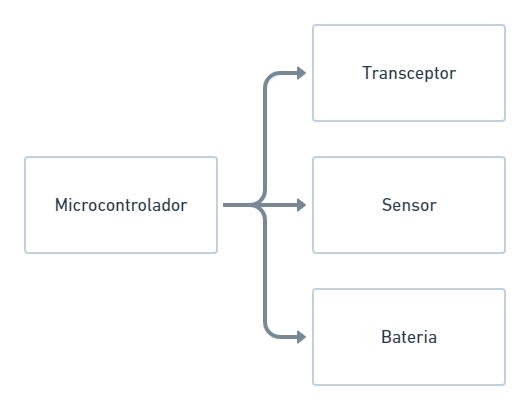
\includegraphics[width=.80\textwidth]{assets/end-node-schematic.png} 
  \caption{Representação da conexão entre os componentes principais do end node (autoral).}
  \label{fig:end-node-schematic} 
\end{figure}

Dentre os diversos sensores disponíveis no mercado para monitoramento de temperatura e umidade, optou-se por escolher um sensor da família DHT, pois é bastante difundida na comunidade, tendo uma boa relação custo benefício. Entre esses sensores, aderimos por usar o DHT22, que consegue captar a temperatura e umidade do ambiente dentro das faixas necessárias para o projeto, com uma boa precisão.

Para o microcontrolador, foi escolhido usar um ATmega328, pois é o utilizado na maioria dos Arduinos, o que nos trás dois grandes benefícios, poder utilizar um arduino como protótipo inicial, por ser fácil de encontrar, de programar e para um protótipo secundário, utilizando o microcontrolador sem o Arduino em si, ainda é possível utilizar o mesmo código, bibliotecas e o mesmo Ambiente de desenvolvimento integrado, IDE, utilizado no primeiro protótipo.

Entre os modelos de transceptores LoRa, o eleito foi o RFM95W, por ser o modelo mais simples e com menos custo e por ser o utilizado dentro do \textit{shield} Arduino, um componente modular feito para adicionar novas funcionalidades a um Arduino de forma fácil e prática, facilitando assim, o desenvolvimento do primeiro protótipo.

Em relação à alimentação do protótipo, é um ponto mais complicado de se analisar e ter uma escolha realmente boa para o caso, mesmo fazendo uma análise aprofundada, apenas teremos uma aproximação da sua eficiência, tal processo é melhor detalhado na seção \ref{metod:end-node:bateria}.

% ---
\subsection{Primeiro Protótipo}
\label{metod:end-node:1-proto}
O primeiro protótipo foi feio com o objetivo de validar os usos das tecnologias, seu alcance, e sua competência em relação a interferências ao longo do trajeto. O consumo energético foi deixado de lado neste protótipo, pois foi utilizado o Arduino e ele possui muitos componentes desnecessários para esta aplicação, que acabam aumentando o gasto energético do dispositivo.

Ele coleta os dando utilizando o sensor DHT-22, formata os dados em uma string e o envia através do LoRa, após isto, ele entra em modo de sono profundo (deep sleep) para economizar bateria por um determinado tempo, ao acordar, ele realiza a medição novamente, e fica nesse ciclo.

\begin{figure}[H]
  \centering
  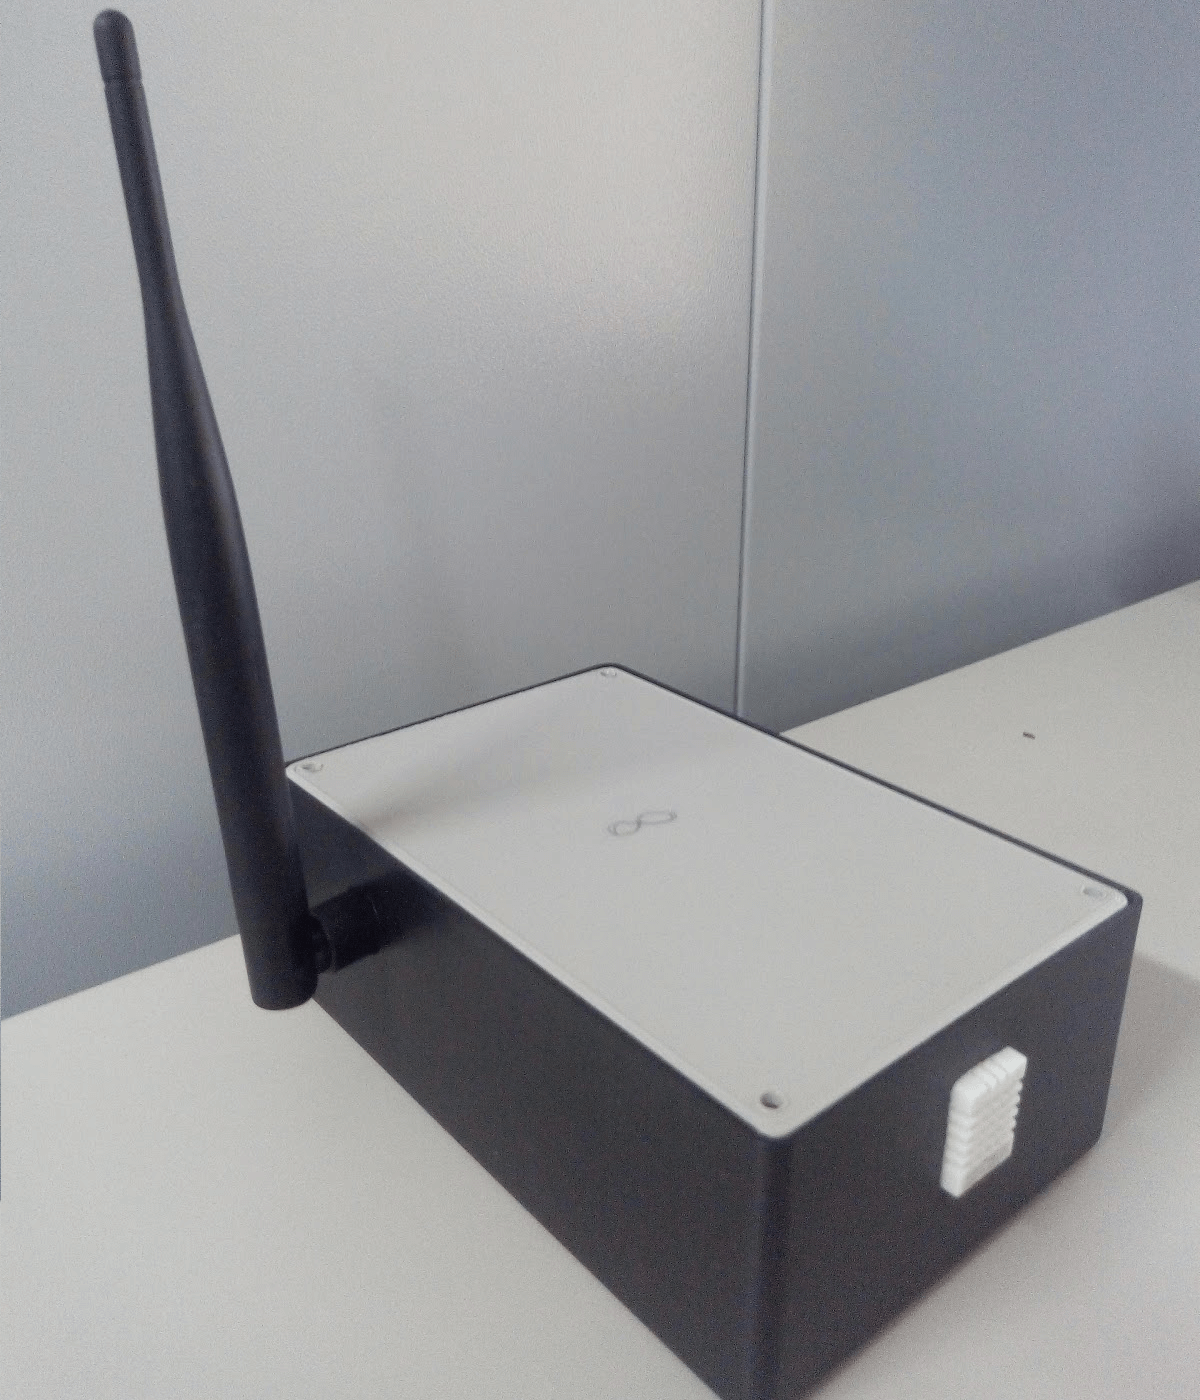
\includegraphics[width=.80\textwidth]{assets/end-node-proto-1.png} 
  \caption{Foto do primeiro protótipo (autoral).}
  \label{fig:end-node-proto-1} 
\end{figure}

% ---
\subsection{Segundo Protótipo}
\label{metod:end-node:2-proto}
O objetivo na construção deste protótipo é construir um dispositivo com um tamanho reduzido e melhorar sua eficiência energética, visando o seu funcionamento por meses com apenas uma pequena bateria. Para conseguir alcançar tais metas, é preciso remover as partes desnecessárias para o funcionamento da aplicação pelo Arduino. Pegando apenas os componentes essenciais, microcontrolador Atmega328, transceptor LoRa RFM95W e o sensor DHT-22, junto com alguns componentes de suporte para fornecer o funcionamento correto, um capacitor de cerâmica de 100pF, dois resistores de 10k Ohms  e um circuito para fornecer o clock para o microcontrolador composto por um cristal oscilador de 16mhz e dois capacitores de cerâmica de 22pF. Tal circuito, como pode ser visto na figura \ref{fig:end-node-proto-2}, foi montado em uma protoboard junto com um conversor USB para serial, para ser possível ver os logs do dispositivo pelo computador.

\begin{figure}[H]
  \centering
  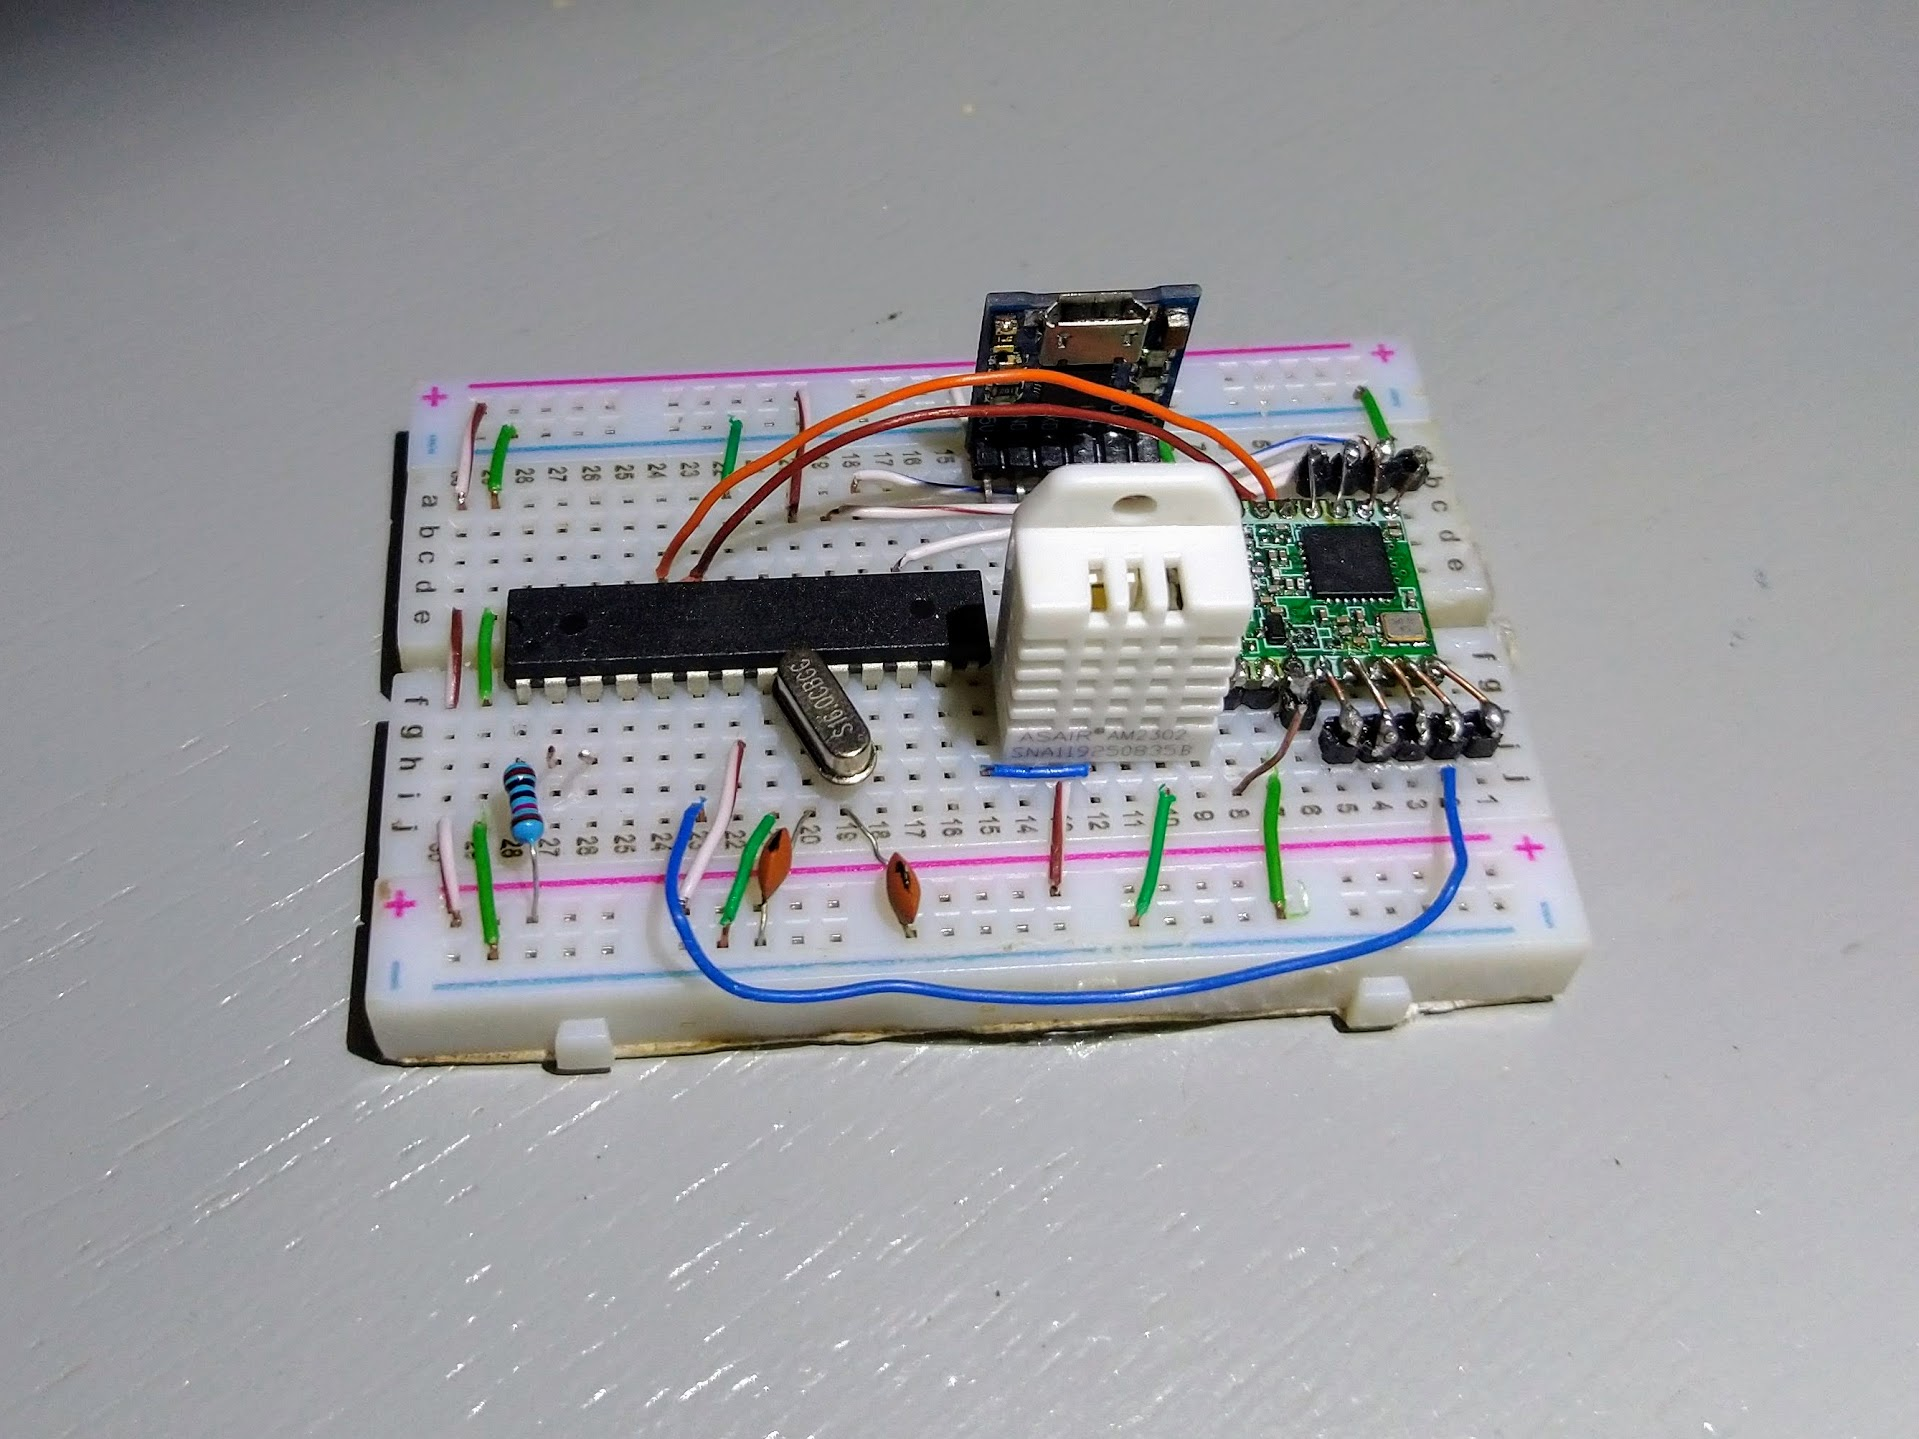
\includegraphics[width=.80\textwidth]{assets/end-node-proto-2.png} 
  \caption{Foto do segundo protótipo (autoral).}
  \label{fig:end-node-proto-2} 
\end{figure}

% ---
\subsection{Escolha da Bateria}
\label{metod:end-node:bateria}
A parte crucial a ser analisada é o consumo de energia, isso é importante para a escolha correta da bateria, que levará a uma duração aceitável do circuito que pode ser meses até anos dependendo da necessidade do produto. É preciso ter em mente as tensões de trabalho dos componentes principais da aplicação, para assim ser possível analisar qual deve ser o valor ideal de trabalho do dispositivo, é possível ver tal informação na tabela \ref{tab:end-node-componentes-volts}, mostrando a tensão mínima e máxima do microcontrolador, transceptor e sensor. Com isto, podemos ver que a tensão de limite superior do dispositivo é referente ao do transceptor LoRa, que funciona até 3,7 Volts, e a tensão de limite inferior, é a do sensor DHT-22, que equivale a 3,3 Volts, se utilizar uma tensão fora deixa faixa, o dispositivo não funcionará corretamente. 

A ideia inicial antes da análise era de usar duas pilhas AA convencionais, entretanto após a análise, tal opção torna-se inviável, pois a tensão máxima de duas baterias AA equivale a 3 Volts, o que é menos do que o mínimo necessário para o sensor DHT-22 funcionar.

\begin{table}[H]
\centering 
\scalebox{1} {
	\begin{tabular}{l | l}
	\textbf{Componente}&\textbf{Tensão de trabalho}\\[5pt] \hline
  \\
	ATmega328&2,7V até 5,5V\\[5pt]
	LoRa RFM95W&1,8V até 3,7V\\[5pt]
	DHT-22&3,3V até 5,5V\\[5pt]
	\end{tabular}
}
\caption{tensão de trabalho dos componentes principais do protótipo (autoral).}
\label{tab:end-node-componentes-volts}
\end{table}

Depois de algumas pesquisas, nos deparamos com uma bateria genérica de referência 18650, que tem o mesmo tamanho de uma AA, é fácil de encontrar em lojas de eletrônica, tem uma capacidade que varia entre 2200mAh e 3400mAh conforme o fabricante, e o mais importante, tem a tensão nominal de 3.7 Volts, o máximo que nosso circuito suporta. Sabendo que os ambientes de armazenagens de vacinas ficaram em torno de -5°C a 8°C, na figura \ref{fig:battery-discharge} podemos ver a linha de descarga da bateria conforme a temperatura de funcionamento, para simplificar os cálculos podemos usar a linha em azul de 0°C. nossa tensão de corte é de 3.3 Volts, analisando o gráfico vemos que a bateria em um ambiente a 0°C a capacidade da bateria cai para aproximadamente 90\%, que equivale há 1980mAh do modelo de 2200mAh.

\begin{figure}[H]
  \centering
  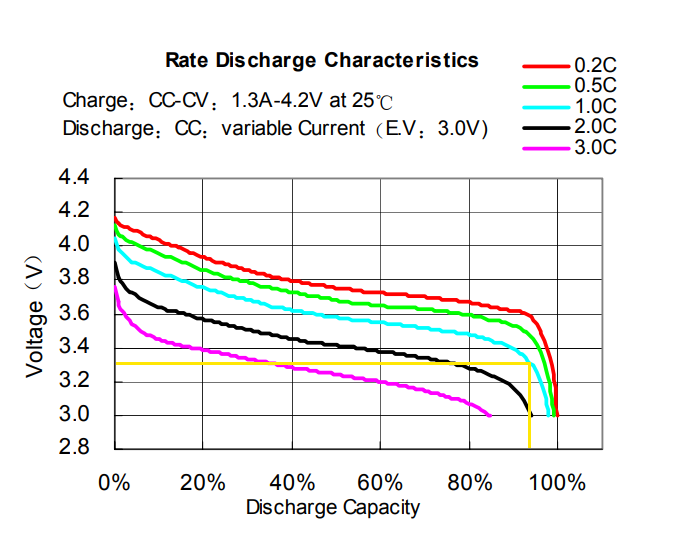
\includegraphics[width=.80\textwidth]{assets/18650-discharge.png} 
  \caption{Descarga da bateria 18650 conforme a temperatura do ambiente (Adaptada de \cite{EEMB201018650}).}
  \label{fig:battery-discharge} 
\end{figure}

% ---
\section{Gateway}
\label{metod:gateway}
O gateway é o dispositivo que fica entre os end nodes e o servidor, e em cada um desses lados, é utilizado uma tecnologia de comunicação diferente, para receber os dados enviados pelos end nodes, se utiliza o LoRa, já para enviar estes dados para o servidor, utiliza-se o HTTP via WiFi. Por isso, é preciso que o gateway possua essas duas tecnologias nele. Felizmente, a Heltec Automation, uma empresa que desenvolve produtos voltada para a IoT utilizando o LoRa, possui um microcontrolador ESP32 que contém tanto o transceptor LoRa, quanto o WiFi, como podemos ver na figura \ref{fig:esp32-lora}. Para programá-lo, foi utilizado a linguagem Arduino, compartilhando assim, a mesma biblioteca entre o end node e o gateway, para o manuseio do transceptor LoRa.

Seu funcionamento segue a seguinte linha, ele fica no aguardo dos pacotes dos end nodes, ao receber um, é realizado uma análise de erro simples, onde é verificado se a formatação do pacote está como esperado, se for detectado algum erro de formatação é enviado para o servidor os valores do RSSI, SNR, o contador do pacote e um atributo booleano marcado como falso, indicando que veio com erro para a seguinte rota, \textit{/packages/:endnodeId}, onde \textit{:endnodeId} é substituído pelo identificador do end node recebido pelo gateway. Se nenhum erro foi detectado, é enviado para a rota do servidor \textit{/sensors/:endnodeId}, os mesmo dados de RSSI, SNR e contador do pacote com o acréscimo dos dados de temperatura e umidade.

\begin{figure}[H]
  \centering
  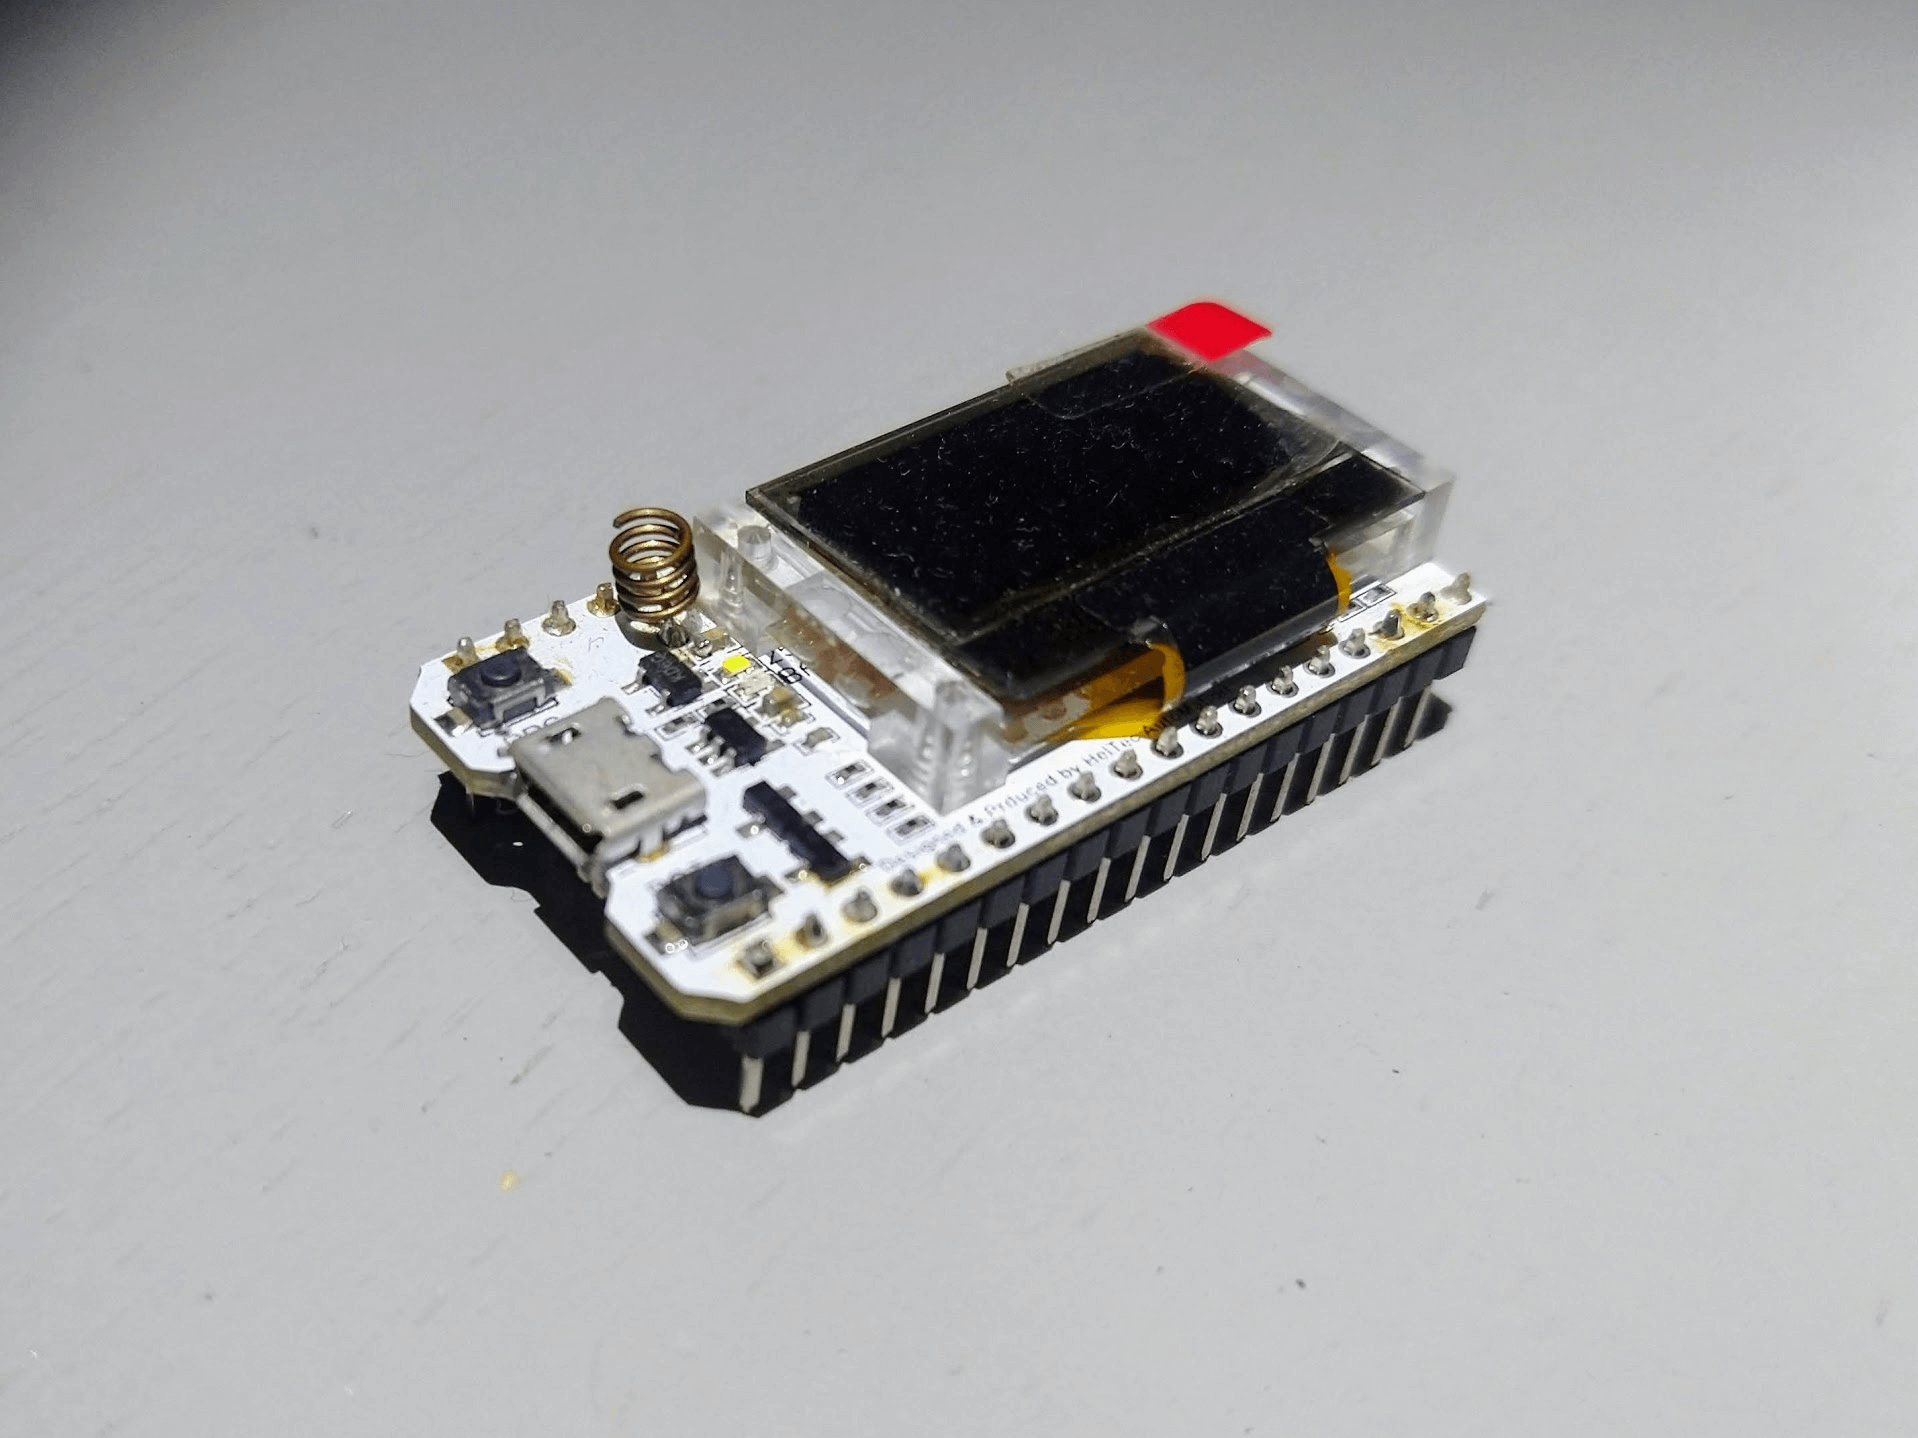
\includegraphics[width=.80\textwidth]{assets/esp32-lora.png} 
  \caption{Foto do ESP32 LoRa da Heltec Automation (autoral).}
  \label{fig:esp32-lora} 
\end{figure}

A configuração do gateway, seu identificador criado pelo servidor e o nome e a senha da rede sem fio que vai ficar conectado, é feita por um ponto de acesso, onde ao liga-lo, ele fornece uma rede sem fio onde é possível acessar seu IP via navegador de Internet, e poder realizar as configurações necessárias.

\begin{figure}[H]
  \centering
  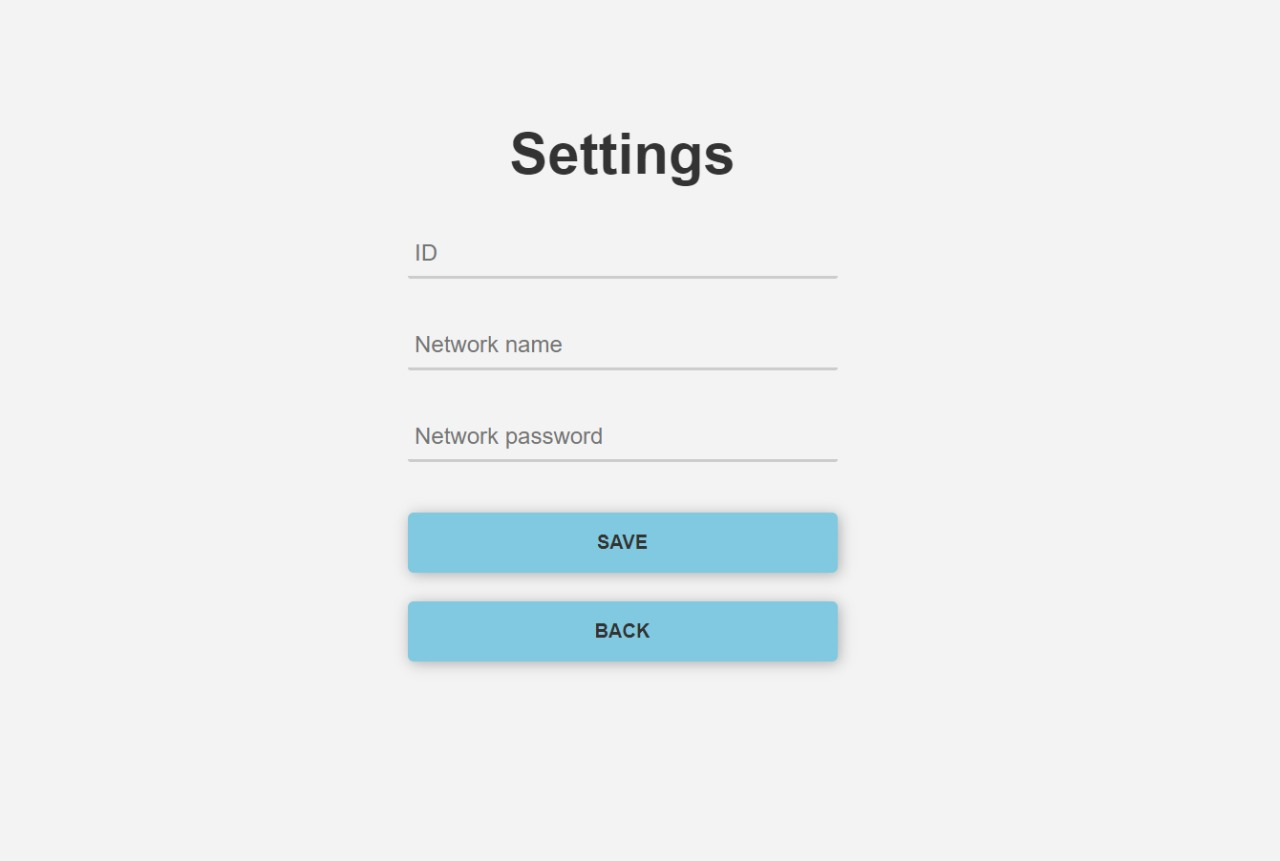
\includegraphics[width=.80\textwidth]{assets/gateway-ap.png} 
  \caption{Página de configuração do gateway (autoral).}
  \label{fig:gateway-ap} 
\end{figure}

% ---
\section{Servidor}
\label{metod:servidor}
Para este projeto, o servidor tem as seguintes responsabilidades: armazenar os dados coletados pelos end-nodes, juntamente com os dados do instituto que está usando a aplicação e dos seus respectivos end-nodes e gateways adquiridos; fornecer rotas para troca de informações com o aplicativo e o gateway, para que possam realizar suas devidas funções.

% ---
\subsection{Padrões de Projetos}
\label{metod:servidor:padroes}
Foi escolhido para desenvolver o servidor, a utilização do Node.js e a linguagem Typescript, se baseando em alguns padrões de softwares, como o Domain-Driven Design (DDD), Test-Driven Development (TDD) e o SOLID visando assim, a construção de um servidor robusto, escalável e de fácil manutenção.

Vale salientar que, esses padrões de softwares, são metodologias de desenvolvimento, e devem ser aplicados de acordo com a demanda da aplicação em construção. Elas são boas práticas, entretanto, dependendo do projeto, alguns pontos podem acabar deixando o processo lendo, e dando pouco benefício, e por isso, nesse projeto, não foi seguido fielmente esses padrões, apenas foi baseado.

Antes de tudo, é preciso definir as regras de negócio básicas do servidor, elas servem para garantir que a aplicação atenda as necessidades esperadas. Para este serviço deve ser possível o usuário se cadastrar, para assim realizar seu \textit{login}, e ter acesso às funcionalidades de cadastrar, editar e remover seus end nodes e seus gateways, além de poder visualizar os dados coletados.

Durante o desenvolvimento de um software, é essencial que a entrega do software funcione corretamente, com qualidade e de acordo com as regras de negócio. Para garantir tais exigências, é importante que se realize testes, tendo em vista identificar possíveis erros antes de chegar aos usuários. Entretanto, realizar testes corretamente é uma tarefa complicada, por isto, existem diversas metodologias, objetivamente facilitar e simplificar os testes dos diferentes componentes de um produto. O TDD é uma dessas metodologias, ela defende o desenvolvimento do teste antes das funcionalidades, garantindo a cobertura completa do código pelos testes.

Junto com o TDD, foi utilizado também o DDD, uma filosofia para auxiliar os desenvolvedores na construção de aplicações complexas de software, ela é referência na organização do código, separando por domínios, de forma isolada. Para poder implementar bem o DDD é preciso definir quais são os domínios da aplicação, analisando as regras de negócio, foi separado em três domínios: end nodes, gateways e usuários.

É preciso também, separar a camada de domínio da aplicação da camada de infraestrutura, a camada de infraestrutura é responsável pelas tecnologias utilizadas para realizar determinada função, por exemplo, a camada de domínio sabe que precisa armazenar os dados dos sensores, mas não é precisar saber onde e nem como, isso é de responsabilidade da camada de infraestrutura.

Para ter uma melhor separação das responsabilidades entre as camadas, é comum utilizar o DDD junto com princípios do SOLID. O SOLID é um acrônimo de 5 princípios da programação orientada a objetos que ajudam o programador a escrever códigos mais limpos, com alta manutenibilidade, separando as responsabilidades e diminuindo acoplamentos.

% ---
\subsection{Banco de Dados}
\label{metod:servidor:db}
É preciso armazenar os dados coletados pelos sensores, para futuras consultas, os dados de transmissão dos pacotes, para utilizar se houver perdas entre as transmissões, e é preciso também, salvar os dados dos usuários e dos seus respectivos produtos cadastrados na plataforma. Tais dados têm suas diferenças, e por isto foi escolhido utilizar banco de dados diferentes para cada um deles.
	
Começando pelos dados coletados pelos sensores e transmitido pelos end-nodes, esses dados são de medidas, coletados com um período curto, e consequentemente, possuem um grande volume. Por isto, foi escolhido utilizar o InfluxDB para armazenar tais dados.

Foi criado duas \textit{measurements} dentro do banco, uma referente aos dados dos sensores e outra aos dados do pacote transmitido, os dois possuindo a mesma  \textit{tag}, o identificador do end node, chamado de endnodeId. Dentro da medida Sensor, foi adicionado dois campos referente a temperatura e umidade do ambiente. Para a medida Package, foi adicionado os campos success, rssi e snr, atributos necessários para saber se o pacote foi entregue com sucesso, a dificuldade de transmitir esse pacote e a relação sinal-ruído. Podemos então ver uma representação do banco na figura \ref{fig:influxdb-model}.

\begin{figure}[H]
  \centering
  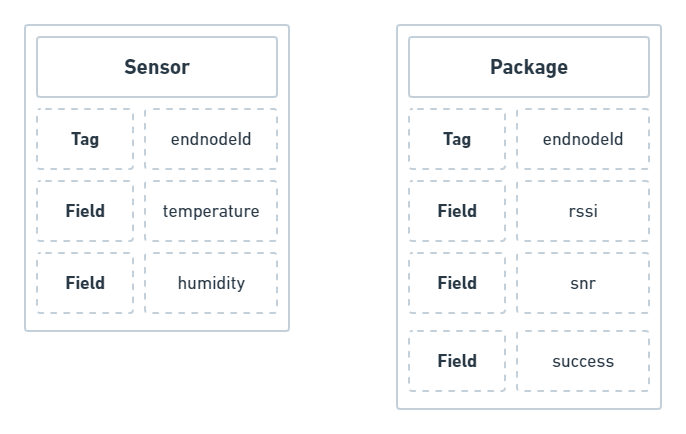
\includegraphics[width=.80\textwidth]{assets/influx-model.png} 
  \caption{Medidas dento do banco de dados InfluxDB (autoral).}
  \label{fig:influxdb-model} 
\end{figure}

Diferentes dos dados que vem dos hardwares, as informações dos usuários e seus dispositivos, não possuem essa demanda alta de escrita e leitura, e mais importante, contém relações entre eles, o que torna banco de dados relacionais uma boa opção para armazenar tais dados. Entre tantos bancos de dados relacionais, foi optado por usar o PostgreSQL por motivos de afinidade.

Cada usuário pode possuir inúmeras gateways e end nodes cadastrados, e cada end node precisa ser vinculado com apenas um gateway. Essas relações entre entre as entidades no postgres representada na figura \ref{fig:postgres-model}, foi pensada olhando tanto para os cenários de pequenos postos de saúde, que tem apenas um local para armazenar seus imunobiológicos, quando para grande hospitais e laboratórios, que pode tem varias salas, com dada sala contendo uma ou mais equipamentos frigoríficos.

\begin{figure}[H]
  \centering
  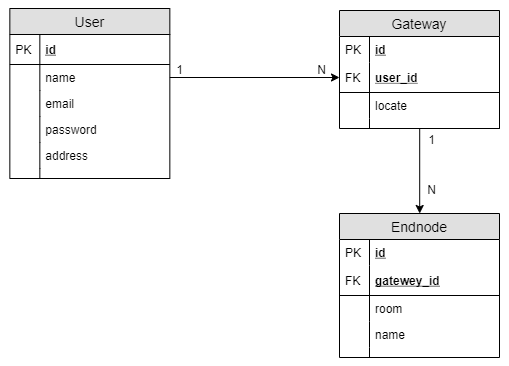
\includegraphics[width=.80\textwidth]{assets/postgres-model.png} 
  \caption{Modelo entidade relacionamento do PostgreSQL (autoral).}
  \label{fig:postgres-model} 
\end{figure}

% ---
\subsection{Containers}
\label{metod:servidor:containers}
Para facilitar o desenvolvimento do servidor, seu deploy e diminuir possíveis problemas por ter várias aplicações rodando na mesma máquina, foi escolhido por conter tantos os bancos de dados quanto a aplicação em si, utilizando o Docker e para facilitar o gerenciamento dos três containers (PostgreSQl, InfluxDB e a aplicação em Node.js), interligando as redes entre eles, foi utilizado o Docker Compose.

Para os bancos de dados, não foi preciso criar as imagens dos containers, dado que são aplicações muito utilizadas e a própria comunidade já oferece algumas opções dependendo da sua finalidade. Entretanto, para a aplicação em si, foi necessário a criação de uma nova imagem, devido algumas configurações extras exigidas pelas tecnologias utilizadas pela aplicação. Tal imagem foi feita baseando-se na versão alpine do node, uma versão mais leve, com apenas as funcionalidades principais.

% ---
\subsection{Deploy}
\label{metod:servidor:deploy}
Entre as opções de servidores na nuvem, foi escolhido por usar a Microsoft Azure para realizar o deploy do servidor. Sua escolha se deu pois a Microsoft oferece uma assinatura para estudantes, o que não teve nenhum custo adicional no desenvolvimento deste protótipo e na realização dos testes.

% ---
\section{Aplicativo móvel}
\label{metod:app}
À necessidade de ter um cliente para que os usuário  possa acessar o histórico de medidas e o gerenciar seus dispositivos, tal cliente poderia ser uma página web, entretanto, tendo em vista o crescimento do uso dos smartphones, tivemos como preferência a criação de uma aplicação móvel, mas especificamente para o sistema operacional Android, devido ao sistema iOS da Apple, restringir seu desenvolvimento para aparelhos da marca, incluindo a necessidade de um computador do mesmo para poder emular um dispositivo móvel com seu sistema operacional.

Tendo em mente as regras de negócios destrinchadas na sessão \ref{metod:servidor:padroes}, a primeira coisa feita foi o desenho das telas utilizando a ferramenta figma, específica para tal tarefa. Ao finalizar os desenhos das telas, partimos para a programação.

Dentre as diversas formas de construir um aplicativo deste porte, a ferramenta escolhida para designar esta função foi o React Native, por motivos de utilizar a mesma linguagem de programação do servidor, typescript, e ter a possibilidade de criar para sistemas iOS futuramente usufruindo do mesmo código.

Pensando na construção de uma aplicação com possibilidades de crescimento altas, foi decidido documentar os componentes que compõem o programa, utilizando a biblioteca Storybook.

\begin{figure}[H]
  \centering
  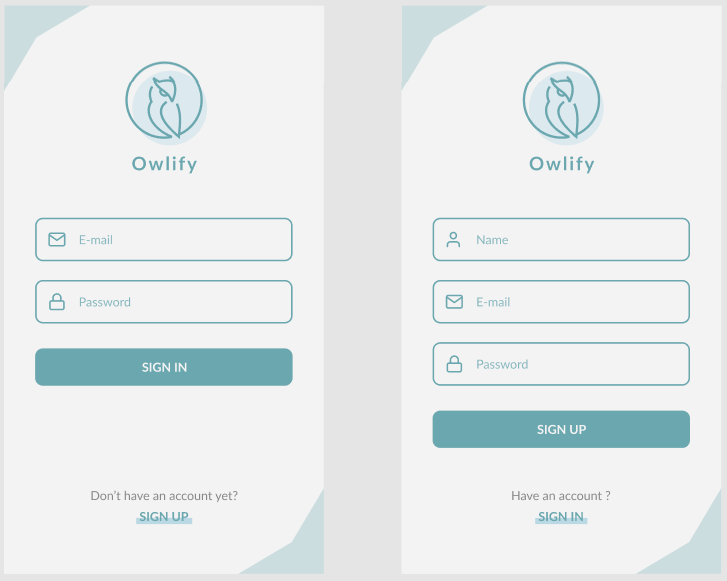
\includegraphics[width=.80\textwidth]{assets/example-app-screens.png} 
  \caption{Desenho das telas de entrar e cadastrar na aplicação (autoral).}
  \label{fig:app-screns-login} 
\end{figure}

% ---
% Finaliza a parte no bookmark do PDF
% para que se inicie o bookmark na raiz
% e adiciona espaço de parte no Sumário
% ---

%\phantompart

% Conclusão (outro exemplo de capítulo sem numeração e presente no sumário)
% \chapter{Considerações Finais}
\label{cap:conclusao}

O presente trabalho apresentou um sistema de monitoração de produtos imunobiológicos, visando o auxílio dos profissionais da saúde em manter a qualidade dos materiais. Tal solução é composta por um aplicativo móvel para o cliente realizar a monitoração, um servidor em nuvem, responsável por concentrar os dados coletados e dos usuários e dos hardwares, que captam as temperaturas e humidades e transmitem para o servidor.

Foi comprovado na sessão \ref{result:transmissao} a efetividade dos hardwares de transmitir os dados coletados em uma distância considerável, cerca de 60 metros, em um ambiente com inúmeros obstáculos causando bastante interferência, proporcionado uma taxa de entrega de pacotes de 78,82\%, um valor alto para o ambiente proposto.
 
Em relação ao custo total de confecção do produto, comprado realizada localmente, ficou  em torno de R\$ 180,00 para o \textit{gateway} e R\$ 97,66 para cada \textit{end node}, a quantidade de end nodes varia conforme a quantidade de ambientes de armazenagem do usuário, uma para cada câmera de conservação de termolábeis. Em relação ao \textit{gateway}, será necessário adquirir outra unidade apenas em caso de algum \textit{end node} ficar localizado em uma distância grande ao ponto do receptor não conseguir receber os pacotes, já que que nas condiçòes estabelecidas, utilizando o LoRaWAN, cada \textit{gateway} pode aguentar, teoricamente, cerca de 62 mil \textit{end node} \cite{lora2021specification}. Considerando a possibilidade de realizar a comprar dos componentes importando da China, o preço dos produtos pode chegar a 50\% a menos em comparação aos preços locais, além de, pensando na produção dos dispositivos em massa, esse preço tende a cair, entretanto, não foi realizado um estudo para saber o quanto de economia teria.

\todo {adicionar um parágrafo falando do consumo energético}

% ---
\section{Sugestões para Trabalhos Futuros}
\label{conclusao:futuros}
Há diversas melhorias que podem ser feitas neste projeto. O LoRa possui um ajuste da potência de transmissão que varia entre +7 dBm a +20 dBm, quanto maior a potência, maior o alcance de transmissão, entretanto, o consumo também cresce. É possível realizar um teste entre esses valores em busca de um melhor balanço entre economia energética e alcance de transmissão, seria interessante também adicionar uma configuração no dispositivo onde o usuário possa escolher qual potência usar, conforme for a sua demanda.

Outra sugestão seria adicionar um nova funcionalidade ao \textit{end nodes} para detectarem que estão em em um ambiente fora do recomendado, ou se teve uma variação considerável em um curto período de tempo da temperatura do ambiente, para que possam emitir um alerta, onde o aplicativo recebe, em tempo real, tal informação.

Olhando para o consumo energético, apesar de termos alcançado um bom resultado, ainda é possível diminuir tal consumo utilizando um \textit{clock} menor, o componente responsável por isso é o cristal oscilador, que neste projeto fui utilizando um de 16 mHz,  entretanto, esta aplicação não necessita dessa \textit{clock} alto, podendo assim utilizar um cristal oscilador de valor menor, inclusive, o próprio Atmega328, possui um clock interno de 1 mHz, que pode ser utilizado no lugar do cristal oscilador, o que traz dois benefícios, uma diminuição dos componentes para o circuito e uma economia de energia.

Um teste interessante a ser realizado, e uma análise em relação a quantidade de dispositivos conectados simultaneamente a um \textit{gateway}, entretanto, necessitaria de muitos dispositivos para realizar tal teste, o que dificultaria na sua realização, considerando que, teoricamente, um \textit{gateway} suporta 1.5 milhões de pacotes por dia, e cada \textit{end node} transmite um pacote por hora, totalizando 24 pacotes por dia.

Este trabalho teve um foco maior na construção do \textit{end node}, o deixou o \textit{gateway} com um grande margem de melhoria, como a construção de um protótipo com apenas as peças necessárias para seu funcionamento, que resultaria em um custo benefício maior e uma economia energética melhor.

Por fim, o servidor foi construído de uma forma modular, que facilita a expansão de novas funcionalidades em trabalhos futuros e pensando na usabilidade do sistema como um todo, tentaria melhorar a usabilidade do aplicativo móvel, em torno do gerenciamento dos dispositivos cadastrados, na atribuição dos identificados aos equipamentos, entre outros.

% ---
% ELEMENTOS PÓS-TEXTUAIS
% ---
\postextual

\bibliography{refs.bib}        % Referências bibliográficas

% ---
% Glossário
% Consulte o manual da classe abntex2 para orientações sobre o glossário.
% \glossary

% \begin{apendicesenv}
  \partapendices  % Imprime uma página indicando o início dos apêndices

  % ---
  \chapter{Um Apêndice}
  \label{ape:apendice1}
  Para criar um novo apêndice utilize o comando chapter, lembre de utilizar label para referenciar.

\end{apendicesenv}
   % Apêndices
% \begin{anexosenv}
  \partanexos % Imprime uma página indicando o início dos anexos

  % ---
  \chapter{Um Anexo}
  \label{ape:anexoI}
  Para criar um novo anexo utilize o comando chapter, lembre de utilizar label para referenciar.

\end{anexosenv}
      % Anexos

%---
% INDICE REMISSIVO
% \phantompart
\printindex

\end{document}
